\documentclass{article}

\usepackage{amsmath}
\usepackage{amssymb}
\usepackage{authblk}
\usepackage{color}
\usepackage{graphicx}
\usepackage{lineno}
\usepackage{natbib}
\usepackage{url}

\linenumbers

\title{Detection of slow slip events using wavelet analysis of GNSS recordings}
\author[1]{Ariane Ducellier}
\author[1]{Kenneth C. Creager}
\author[1]{David A. Schmidt}
\affil[1]{University of Washington, Department of Earth and Space Sciences, Box 351310, 4000 15th Avenue NE Seattle, WA 98195-1310}
\date{}

\begin{document}

\maketitle

\section*{Key points}

\begin{itemize}
\item We use a wavelet-based signal processing method to detect transients in GNSS data, such as slow slip events.
\item There is a good correlation between detections using GNSS data and independent detections using seismic data.
\item The method could be applied in regions where no tremor are detected in conjunction with slow slip events.
\end{itemize}

\newpage

\section*{Abstract}

In many places, tectonic tremor is observed in relation to slow slip and can be used as a proxy to study slow slip events of moderate magnitude where surface deformation is hidden in Global Navigation Satellite System (GNSS) noise. However, in subduction zones where no clear relationship between tremor and slow slip occurrence is observed, these methods cannot be applied, and we need other methods to be able to better detect and quantify slow slip. Wavelets methods such as the Discrete Wavelet Transform (DWT) and the Maximal Overlap Discrete Wavelet Transform (MODWT) are mathematical tools for analyzing time series simultaneously in the time and the frequency domain by observing how weighted differences of a time series vary from one period to the next. In this paper, we use wavelet methods to analyze GNSS time series and seismic recordings of slow slip events in Cascadia. We use detrended GNSS data, apply the MODWT transform and stack the wavelet details over several nearby GNSS stations. As an independent check on the timing of slow slip events, we also compute the cumulative number of tremor in the vicinity of the GNSS stations, detrend this signal, and apply the MODWT transform. In both time series, we can then see simultaneous waveforms whose timing corresponds to the timing of slow slip events. We assume that there is a slow slip event whenever there is a positive peak followed by a negative peak in the wavelet signal. We verify that there is a good correlation between slow slip events detected with only GNSS data, and slow slip events detected with only seismic data for northern Cascadia. The wavelet-based detection method detects well events of magnitude higher than 6 as determined by independent event catalogs (e.g. ~\citep{MIC_2019}).

\section{Introduction}

Slow slip events are a new feature discovered in the last two decades in many subduction zones thanks to recordings of the displacement of Earth's surface by dense Global Navigation Satellite System (GNSS) networks. As with ordinary earthquakes, slow slip events represent slip on a fault, for instance the plate boundary between a tectonic plate subducting under another tectonic plate. However, they take a much longer time (several days to several years) to happen relative to ordinary earthquakes. They have a relatively short recurrence time (months to years) compared to the recurrence time of regular earthquakes (up to several hundreds of years), allowing scientists to observe and study many complete event cycles, which is typically not possible to explore with traditional earthquake catalogs ~\citep{BER_2011}. A slow slip event on the plate boundary is inferred to happen when there is a reversal of the direction of motion at GNSS stations, compared to the secular interseismic motion. Slow slip events have been observed in many places, such as Cascadia, Nankai (southwest Japan), Alaska, Costa Rica, Mexico, and New Zealand ~\citep{BER_2011,AUD_2016}. \\

In many places, tectonic tremor is also observed in relation to slow slip, but it is more abundant in some places. Tremor is a long (several seconds to many minutes), low amplitude seismic signal, with emergent onsets, and an absence of clear impulsive phases. Tectonic tremor have been explained as a swarm of small, low-frequency earthquakes (LFEs) ~\citep{SHE_2007_nature}, which are small magnitude earthquakes (M $\sim$ 1) for which frequency content (1-10 Hz) is lower than for ordinary earthquakes (up to 20 Hz). In subduction zones such as Nankai and Cascadia, tectonic tremor observations are spatially and temporally correlated with slow slip observations ~\citep{OBA_2002,ROG_2003}. Due to this correlation, these paired phenomena have been called Episodic Tremor and Slip (ETS). However, this is not always the case. For instance, in northern New Zealand, tremor are more challenging to detect, and seem to be located downdip of the slow slip on the plate boundary ~\citep{TOD_2016}. In Alaska, the tremor zone only partially overlaps the long-term slow slip zone and there does not appear to be any temporal correlation between tremor and slow slip occurrence ~\citep{WEC_2016}. \\

In Cascadia, there are robust signals in both GNSS and tremor. This is also the case in Nankai, where tiltmeters are used instead of GNSS. It is thus possible to use tremor as a proxy to observe slow slip events that are not directly observed in the GNSS data. For instance, ~\citet{AGU_2009} studied 23 ETS events in Cascadia with more than 50 hours of tectonic tremor. For all these events, they computed both the GPS-estimated moment release and the cumulative number of hours of tectonic tremor recorded. They observed a linear relationship between moment release and number of hours of tremor for ETS events of moment magnitude 6.3 to 6.8. Based on this linear relationship, it is possible to infer the existence of smaller slow slip events of magnitude 5-6 occurring simultaneously with smaller tremor bursts of duration 1 to 50 hours occurring in between the big ETS events, and for which there is no detectable signal in the GPS data. \\

~\citet{FRA_2016} divided GPS time series observations from Cascadia and Guerrero, Mexico, into two groups: the first group contains days with abundant tremor and LFEs, the second group contains days when the number of tremor or LFEs is lower than a threshold. He then stacked separately the two groups of daily observations and observed a cumulative displacement in the direction corresponding to the loading period when few tremor or LFEs are observed and the surface deformation corresponds to the secular plate motion. He also observed a cumulative displacement in the opposite direction corresponding to the release period when tremor and LFEs are observed. He was thus able to observe a reverse displacement corresponding to smaller slow slip events not directly observable in the GPS data for individual events. \\

However, these methods cannot be applied to detect slow slip events in places where tremor and slow slip occurrence are not well spatially and temporary correlated, tremor is not abundant, or the seismic network is not robust enough. We thus need other methods to be able to better detect and quantify slow slip. \\

Wavelets methods such as the Discrete Wavelet Transform (DWT) are mathematical tools for analyzing time series simultaneously in the time and the frequency domain by observing how weighted differences of a time series vary from one period to the next. Wavelet methods have been widely used for geophysical applications (e.g. ~\citep{KUM_1997}). However, few studies have used wavelet methods to analyze recordings of slow slip, and their scope was limited to the detection of the bigger (magnitude 6-7) short-term (a few weeks) events ~\citep{SZE_2008,OHT_2010,WEI_2012,ALB_2019}. \\

~\citet{SZE_2008} determined the timing and the amplitude of 34 slow slip events throughout the Cascadia subduction zone between 1997 and 2005 using wavelets. They modeled the GPS time series by the sum of a linear trend, annual and biannual sinusoids representing seasonal effects, Heaviside step functions corresponding to earthquakes and hardware upgrades, and a residual signal. They then applied a Gaussian wavelet transform to the residual time series to get the exact timing of slow slip at each GPS station. The idea is that the wavelet transform allows us to analyze the signal both in the time and the frequency domains. A sharp change in the signal will be localized and seen at all levels of the wavelet decomposition, contrary to what happens with the periodic sinusoids of the Fourier transform. \\

Instead of using wavelets in the time domain, ~\citet{OHT_2010} used 2D wavelet functions in the spatial domain to detect slow slip events. They designed the Network Stain Filter (NSF) to detect transient deformation signals from large-scale geodetic arrays. They modeled the position of the GPS station by the sum of the secular velocity, a spatially coherent field, site-specific noise, reference frame errors, and observation errors. The spatial displacement field is modeled by the sum of basis wavelets with time-varying weights.  Their method has been successfully used to detect a transient event in the Boso peninsula, Japan, and a slow slip event in the Alaska subduction zone ~\citep{WEI_2012}. \\

Finally, ~\citet{ALB_2019} used hourly water level records from four tide gauges in the Juan de Fuca Straight and the Puget Sound to determine relative vertical displacements associated with ETS events between 1996 and 2011. Their main idea is that the tidal level measured at a given gauge is the sum of a noise component at multiple timescales (tides, ocean and atmospheric noise) and an uplift signal due to the ETS events. The noise component is assumed to be coherent between all tidal gauges, while the tectonic uplift signal is different provided that the gauges are far enough from each other. By stacking the tidal records after removing tides, the uplift signals cancel each other while the noise signal is amplified. By stacking the details of the DWT decomposition, instead of stacking the raw tidal record, each of the components of the noise at different time scales is retrieved and can then be removed from the raw records to obtain the uplift signal. The authors were then able to clearly see a difference in uplift between the two tidal gauges at Port Angeles and Port Townsend. \\

In our study, we use a similar approach to previous studies with a different reasoning. We only stack signals at nearby GPS stations, assuming that the longitudinal displacement due to the ETS events will then be the same at each of the GPS stations considered. We suppose that some of the noise component is different at each GPS station and will be eliminated by the stacking. Finally, we assume that the noise and the longitudinal displacement due to the ETS events and the secular plate motion have different time scales, so that the wavelet decomposition will act as a bandpass filter to retrieve the displacement signal and highlight the ETS events. We use wavelet methods to analyze GPS and seismic recordings of slow slip events in Cascadia. Our objective is to verify that there is a good correlation between slow slip events detected with only GNSS data, and slow slip events detected with only seismic data. We thus want to demonstrate that the wavelet-based detection method can be applied to detect slow slip events that may currently be obscured using standard methods. \\

\section{Data}

We focused our study on northwest Washington State. For the GNSS data, we used the GPS time series provided by the Pacific Northwest Geodetic Array, Central Washington University. These are network solutions in ITRF2008 with phase ambiguities resolved. Solutions are computed with JPL/NASA orbits and satellite clocks. North, East, and Vertical directions are available. However, as the direction of the secular plate motion is close to the East direction, we only used the East direction of the GPS time series for the data analysis, as it has the best signal-to-noise ratio. The wavelet method works best with data with zero mean, and no sharp discontinuities; so we use the cleaned dataset, that is GPS times series with linear trends, steps due to earthquakes or hardware upgrades, and annual and semi-annual sinusoids signals simultaneously estimated and removed following ~\citet{SZE_2004}. For the seismic data, we used the tremor catalog from \textcolor{red}{reference for the catalog. The following is to be modified. the Pacific Northwest Seismic Network (PNSN) ~\citep{WEC_2010}. Tremor were detected and located using waveform envelope correlation and clustering and a centroid location is available for every given five-minute time window when tremor was detected. As the catalog starts in August 2009, we only looked at GPS data recorded in 2009 or later.} \\

\section{Method} 

\subsection{The Maximal Overlap Discrete Wavelet Transform}

The Discrete Wavelet Transform (DWT) is an orthonormal transform that transforms a time series $X_t \left( t = 0, \cdots , N - 1 \right)$ into a vector of wavelet coefficients $W_i \left( i = 0 , \cdots , N - 1 \right)$. If we denote $J$ the level of the wavelet decomposition, and the number of observations is equal to $N = n * 2^J$, where $n$ is some integer higher or equal to 1, the vector of wavelet coefficients can be decomposed into $J$ wavelet vectors $W_j$ of lengths $\frac{N}{2}$, $\frac{N}{4}$, ... , $\frac{N}{2^J}$, and one scaling vector $V_J$ of length $\frac{N}{2^J}$. Each wavelet vector $W_j$ is associated with changes on time scale $\tau_j = dt 2^{j - 1}$, where $dt$ is the time step of the time series, and corresponds to the filtering of the original time series with a filter with nominal frequency interval $\lbrack \frac{1}{dt 2^{j + 1}} ; \frac{1}{dt 2^j} \rbrack$. The scaling vector $V_J$ is associated with averages in time scale $\lambda_J = dt 2^J$, and corresponds to the filtering of the original time series with a filter with nominal frequency interval $\lbrack 0 ; \frac{1}{dt 2^{j + 1}} \rbrack$. Wavelet vectors can be further decomposed into details and smooths, which are more easily interpretable. We define for $j = 1 , \cdots , J$ the $j$th wavelet detail $D_j$, which is a vector of length $N$, and is associated to time scale $\tau_j = dt 2^{j - 1}$. Similarly, we can define for $j = 1 , \cdots , J$ the $j$th wavelet smooth $S_j$, which is a vector of length $N$, and is associated to scales $\tau_{j + 1} = dt 2^{j + 1}$ and higher. The basic idea is to reapply to $W_j$ the wavelet filter that was used to construct $W_j$ from the initial time series $X$. Together, the details and the smooths define the multiresolution analysis (MRA) of $X$:

\begin{linenomath*}
\begin{equation}
X = \sum_{j = 1}^{J} D_j + S_J
\end{equation}
\end{linenomath*}

The DWT presents several disadvantages. First, the length of the time series must be a multiple of $2^J$ where $J$ is the level of the DWT decomposition. Second, the time step of the wavelet vector $W_j$ is $dt 2^j$, which may not correspond to the time when some interesting phenomenon is visible on the original time series. Third, when we circularly shift the time series, the corresponding wavelet coefficients, details and smooths are not a circularly shifted version of the wavelet coefficients, details and smooths of the original time series. Thus, the values of the wavelet coefficients, details and smooths are strongly dependent on the time when we start experimentally gathering the data. Finally, when we filter the time series to obtain the details $D_j$ and smooths $S_j$, we introduce a phase shift, which makes it difficult to line up meaningfully the features of the MRA with the original time series. \\

To overcome the disadvantages described above, we use instead the Maximal Overlap Discrete Wavelet Transform (MODWT). The MODWT transforms the time series $X_t \left( t = 0, ... , N - 1 \right)$ into J wavelet vectors $\widetilde{W}_j \left( j = 1 ,  \cdots , J \right)$ of length $N$ and a scaling vector $\widetilde{V}_J$ of length $N$. As is the case for the DWT, each wavelet vector $\widetilde{W}_j$ is associated with changes on scale $\tau_j = dt 2^{j - 1}$, and corresponds to the filtering of the original time series with a filter with nominal frequency interval $\lbrack \frac{1}{dt 2^{j + 1}} ; \frac{1}{dt 2^j} \rbrack$. The scaling vector $\widetilde{V}_J$ is associated with averages in scale $\lambda_J = dt 2^J$, and corresponds to the filtering of the original time series with a filter with nominal frequency interval $\lbrack 0 ; \frac{1}{dt 2^{j + 1}} \rbrack$. As is the case for the DWT, we can write the MRA:

\begin{linenomath*}
\begin{equation}
X = \sum_{j = 1}^{J} \widetilde{D}_j + \widetilde{S}_J
\end{equation}
\end{linenomath*}

The MODWT of a time series can be defined for any length $N$. The time step of the wavelet vectors $\widetilde{W}_j$ and the scaling vector $\widetilde{V}_J$ is equal to the time step of the original time series. When we circularly shift the time series, the corresponding wavelet vectors, scaling vector, details and smooths are shifted by the same amount. The details and smooths are associated with a zero phase filter, making it easy to line up meaningfully the features of the MRA with the original time series. The wavelet methods for time series analysis are explained in a more detailed way in ~\citep{PER_2000}). \\

\subsection{Application to synthetic data}

To illustrate the wavelet transform method, we first apply the MODWT to synthetic data. As slow slip events occur in Cascadia on a regular basis, every twelve to eighteen months, we create a synthetic signal of period $T = 500$ days. To reproduce the ground displacement observed on the longitudinal component of GPS stations in Cascadia, we divide each period into two parts: In the first part of duration $T - N$, the displacement is linearly increasing and corresponds to the inter seismic plate motion in the eastern direction; in the second part of duration $N$, the displacement is linearly decreasing and corresponds to a slow slip event on a reverse fault at depth triggering a ground displacement in the western direction. To see the effect of the duration of the slow slip event, we use different values for $N = 5, 10, 20, 40$ days. The amplitude of the set is normalized to 1. Figure 1 shows the synthetics, the details $D_j$  of the wavelet decomposition for levels 1 to 10, and the smooth $S_{10}$ for the four durations of a slow slip event. \\

The ramp-like signal is transformed through the wavelet filtering into a waveform with first a positive peak and then a negative peak. The shape of the waveform is the same for every level of the wavelet decomposition, but the width of the waveform increases with the scale level. For the 8th level of the wavelet decomposition, the width of the waveform is nearly as large as the time between two events. At larger scales, the waveforms start to merge two contiguous events together, and make the wavelet decomposition less interpretable. For an event of duration 5 days, the wavelet details at levels higher than 3 have a larger amplitude than the wavelet details at lower scales. For an event of duration 10 days, the wavelet details at levels higher than 4 have a larger amplitude than the wavelet details at lower scales. For an event of duration 20 days, the wavelet details at levels higher than 5 have a larger amplitude than the wavelet details at lower scales. For an event of duration 40 days, the wavelet details at levels higher than 6 have a larger amplitude than the wavelet details at lower scales. Thus, the scale levels at which an event is being seen in the wavelet details give us an indication about the duration (and the magnitude) of the slow slip event. The big slow slip events of magnitude 6-7 typically trigger a signal that lasts about one week at an individual GPS station, and the whole event lasts several weeks. We expect them to start being visible at the level 5 of the wavelet decomposition, but to not be noticeable at lower time scales. \\

\subsection{MODWT of GPS and tremor data}

The DWT and MODWT methods must be used on a continuous time series, without gaps in the recordings. To deal with the gaps in the GNSS recordings, we simply replace the missing values by interpolation. The value for the first day for which data are missing is equal to the mean of the five days before the gap. The value for the last day for which data are missing is equal to the mean of the five days after the gap. The remaining missing values are computed by doing a linear interpolation of the first and the last values and adding a Gaussian noise component with mean zero and standard deviation equal to the standard deviation of the whole time series. The straight line starts at and ends at . We verify how the wavelet details may be affected by looking at a GPS time series without missing values and compared the wavelet details with and without removing some data points. Station PGC5 recorded continuous 1390 days between 2009 and 2013 without any missing values. We first computed the wavelet details without missing values. Then, we removed ten neighboring values, replaced them using the method described above (linear interpolation plus Gaussian noise), and computed the wavelet details with the replaced values. Figure 2 shows a comparison of the two wavelet details for two different locations of the missing values. We can see that there are visible differences in the time series itself, and in the details at the smallest levels of the wavelet decomposition. However, the differences between the wavelet details with and without missing values get smaller and smaller with increasing levels of details, and are barely visible for the levels that are most relevant (levels 6 and above). We thus conclude that we can easily replace the missing values in the GNSS time series without introducing false detections of slow slip events. \\

We then applied the wavelet filtering to real GPS data. Figure 3 shows the longitudinal displacement for GPS station PGC5, located in southern Vancouver Island, the details of the wavelet decomposition for levels 1 to 8, and the smooth. In the data, we can see a sharp drop in displacement whenever there is a documented slow slip event. For levels 5 to 8, which correspond to time scales 16, 32, 64 and 128 days, we can see in the details a positive peak followed by a negative peak whenever there is a drop in displacement in the data. We thus verify that the wavelet method can detect steps in the time series associated with slow slip events. \\

To increase the signal-to-noise ratio and better detect slow slip events, we stack the signal from several neighboring GPS stations. We choose to focus on GPS stations located close enough to the tremor zone to get a sufficiently high amplitude of the slow slip signal. We choose 16 points along the 40 km depth contour of the plate boundary (model from ~\citet{PRE_2003}) with spacing equal 0.1 degree in latitude (red triangles on Figure 4). Then we took all the GPS stations located in a 50 km radius for a given point, compute the wavelet details for the longitudinal displacement of each station, and stack each detail over the GPS stations. We thus have a stacked detail for each level 1 to 10 of the wavelet decomposition. \\

To assess the success of the wavelet decomposition for detecting slow slip events in GPS time series, we validate the approach by comparing to an independent proxy for ETS events. We took all the tremor epicenters located within a 50 km radius centered on one of the 16 locations marked by red triangles on Figure 3. Then we computed the cumulative number of tremor within this circle. Finally, we removed a linear trend from the cumulative tremor count, and applied the wavelet transform. Figure 5 shows an example of the wavelet decomposition for the third northernmost location on Figure 4 (which is closest to GPS station PGC5). Contrary to what happens for the GPS data, we see a sharp increase in the time series whenever there is a tremor episode, which translates into a negative peak followed by a positive peak in the wavelet details.

\section{Results}

We stacked the 8th level detail of the wavelet decomposition of the displacement over all the GPS stations located in a 50 km radius of a given point, for the 16 locations indicated in Figure 3. The result is shown in the top panel of Figure 6, where each line represents one of the locations along strike. To better highlight the peaks in the wavelet details, we highlighted in red the time intervals where the amplitude of the stacked detail is higher than a threshold, and in blue the  time intervals where the amplitude of the stacked detail is lower than minus the threshold. To compare the GPS signal with the tremor signal, we plotted the 8th level detail of the wavelet decomposition of the tremor count on the bottom panel of Figure 6. We multiplied by -1 the cumulative tremor count for the wavelet decomposition in order to be able to match positive peaks with positive peaks and negative peaks with negative peaks. In the tremor catalog from \textcolor{red}{reference?}, there are 17 tremor events with more than 150 hours of tremor recorded. The events are summarized in Table 1. The time of the event is the start date plus half the duration of the event. \\

Although the latitudinal extension of the events is not always the same for the GPS data and for the tremor data, we identify the same 13 events in both 8th wavelet decompositions for the 8th level: January 2007, May 2008, May 2009, August 2010, August 2011, September 2012, September 2013, August-November 2014, January 2016, March 2017, June 2018, March-November 2019, and October 2020-January 2021. Although there are two events in the tremor catalog in August 2014 and November 2014, these two events are not distinguishable in the 8th level details and look more like a single event slowly propagating from South to North. The same phenomenon is observed in 2019 when two tremor events in March and November 2019 are merged into a single event propagating slowly from South to North. In 2020-2021, the wavelet decomposition of the tremor shows one event in the south in October-November 2020 and one event in the North in January 2021, but in the wavelet decomposition of the GPS data, these three events look like a single event propagating slowly from South to North. \\

A similar comparison is shown for the wavelet decomposition of the GPS data and the wavelet decomposition of the tremor count data for the 7th level and the 6th level respectively (Figures 7 and 8). The events are harder to see in the 7th level than in the 8th level, both for the GPS data and the tremor count data. The wavelet decomposition is more noisy for the GPS data between 2010 and 2012, but it does not seem that there are more slow slip events visible in the 7th level. \\

For the 6th level detail, we see an additional event in the South in Fall 2009 that is present both in the GPS and the tremor data. It may correspond to the northern extent of a big ETS event occurring in Fall 2009 south of the study area (event 19 in the ~\citet{MIC_2019} catalog). There are three small signals in the GPS data in Spring 2012, Fall 2017, and Winter 2020 that are not present in the tremor data, and are probably false detections. To summarize, we assume that true detections are events present in both GPS and tremor time series, and false detections are events present in the GPS but not in the tremor time series. Then, all the 13 events present on the 8th level detail of the wavelet decomposition are true detections and 14 of the 17 events present on the 6th level detail of the wavelet decomposition are true detections. \\

\section{Discussion}

To better evaluate the number of true and false detections, we convert the wavelet details into binary time series. If the absolute value of the wavelet detail is higher that a threshold, we replace the value by 1 (for positive values) or -1 (for negative values), otherwise we replace the value by 0. We do this on both the wavelet details of the GPS data and of the tremor data. Then we decide that if both the GPS and the tremor time series take the value 1 (or both take the value -1), we have a true detection (true positive, TP). If the GPS and the tremor time series have opposite signs, or if the absolute value of the GPS time series is 1 but the value of the tremor time series is 0, we have a false detection (false positive, FP). If both time series take the value 0, we do not have detection (true negative, TN). If the GPS time series take the value 0, but the absolute value of the tremor time series is 1, we miss a detection (false negative, FN). We then define the sensitivity (true positive rate) and the specificity (equal to 1 minus the false positive rate) as:

\begin{equation}
\begin{aligned}
\text{sensitivity} &= \frac{TP}{TP + FN} \\
\text{specificity} &= \frac{TN} {TN + FP}
\end{aligned}
\end{equation}

We can then evaluate the quality of the detections obtained with our method by plotting a receiver operating characteristic curve (ROC curve). The ROC curve is widely use for binary classification problems in statistics and machine learning. We calculate an ROC value by varying the values of the threshold (here the two thresholds used to convert the GPS and the tremor time series into binary time series), computing the corresponding values of the true positive rate and the false positive rate (equal to 1 minus the specificity), and plotting the true positive rate as a function of the false positive rate. If the classification was made randomly, all the points would fall on the first diagonal. If the classifier was perfect, the corresponding point would fall on the top left corner of the graph with true positive rate equal to 1 and false positive rate equal to 0. The bigger the area under the curve, the better the classification method is. \\

As the slow slip events are better seen on levels 6, 7 and 8 of the wavelet decomposition, we first add the wavelet details corresponding to levels 6 to 8, and transform the resulting time series into a binary time series. We apply this transform to both the GPS and the tremor time series with varying thresholds. We then plot the ROC curve on Figure 9, each dot representing a different threshold. The corresponding sums of the wavelet details for the GPS data and the tremor data are shown on Figure 10. We can see that there is a trade-off between sensitivity and specificity as we vary the threshold. If we decrease the false positive rate, we also decrease the number of true events detected. If we increase the number of true events detected, we also increase the false positive rate. In Figure 10, we have chosen thresholds for the GPS time series and the tremor time series such that the specificity is higher than 0.75, and the sensitivity is the highest possible, that is we have chosen the thresholds corresponding to the dot that is farthest from the diagonal, which is random. \\

In addition to the magnitude 6 events discussed above,  ~\citet{MIC_2019} have also identified several magnitude 5 events using a variational Bayesian Independent Component Analysis (vbICA) decomposition of the signal. As we expect smaller magnitude events to be more visible at smaller time scales of the wavelet decomposition (level 5), we verify for all these events whether a signal can be seen at the same time as the time given in their catalog. Most of these magnitude 5 events are also sub-events of bigger magnitude 6 events. Table 2 summarizes for each event its timing, its number and its magnitude as indicated in the catalog from ~\citet{MIC_2019}, and whether it is part of a bigger magnitude 6 event. Figure 11 shows the 5th level detail wavelet decomposition of the GPS data. Red lines show the timing of the big ETS events from Table 1, and blue lines show the timing of the small slow slip events from Table 2. \\

All 14 events that are sub-events of a bigger event are visible at level 5. However, this may be because the bigger events are clearly seen at levels 6 to 8, and also at smaller time scales. The one small event that is not part of a bigger event (Winter 2009) is visible at level 5 of the wavelet decomposition. However, some other events that are not in the catalog of ~\citet{MIC_2019}'s catalog are also visible in late 2007, early 2010, early 2012, and late 2016. Therefore, it is difficult to differentiate between a true detection and a false detection, and to conclude whether the method can indeed detect events of magnitude 5.

\section{Conclusion}

In this paper, we develop and test a new approach for detecting transient events in GPS time series, such as slow slip events. We used wavelet methods to analyze GNSS time series and seismic recordings of slow slip events in Cascadia. We used detrended GNSS data, applied the MODWT transform, and stacked the wavelet details over several nearby GNSS stations. As an independent check on the timing of slow slip events, we also computed the cumulative number of tremor in the vicinity of the GNSS stations, detrended this signal, and applied the MODWT transform. In both time series, we could then see simultaneous waveforms whose timing corresponds to the timing of slow slip events. We assumed that there is a slow slip event whenever the wavelet signal gets above a threshold. We verified that there is a good correlation between slow slip events detected with only GNSS data, and slow slip events detected with only seismic data. The wavelet-based detection method detects all events of magnitude higher than 6 as determined by independent event catalogs (e.g. ~\citep{MIC_2019}). We detected signals in the GPS data that could be magnitude 5 events, but it is not easy to differentiate between true detections and false detections.

\section*{Data and Resources}

The GPS recordings used for this analysis can be downloaded from the PANGA website ~\citep{PANGA} \url{http://www.panga.cwu.edu/}. \textcolor{red}{Reference for tremor catalog}. The Python scripts used to analyze the data and make the figures can be found on the first author's Github account \url{https://github.com/ArianeDucellier/slowslip}. Figure 4 was created using GMT ~\citep{WES_1991}.

\section*{Acknowledgements}

This work was funded by the grant from the National Science Foundation XXX. A.D. would like to thank Pr Donald Percival for introducing her to wavelet methods during his excellent class taught at University of Washington.   

\section*{Declaration of Competing Interests}

The authors declare no competing interests.

\bibliographystyle{plainnat}
\bibliography{bibliography}

\newpage

\section*{Addresses}

Ariane Ducellier. University of Washington, Department of Earth and Space Sciences, Box 351310, 4000 15th Avenue NE Seattle, WA 98195-1310. \\

Kenneth C. Creager. University of Washington, Department of Earth and Space Sciences, Box 351310, 4000 15th Avenue NE Seattle, WA 98195-1310. \\

David A. Schmidt. University of Washington, Department of Earth and Space Sciences, Box 351310, 4000 15th Avenue NE Seattle, WA 98195-1310.

\newpage

\section*{Tables}

\begin{table}[hbt!]
\caption{Episodic Tremor and Slip events with M > 6 identified by MODWT in both the GPS and the tremor data. The duration and the number of tremor are from the tremor catalog of \textcolor{red}{reference?}. The event number and the magnitude are from the slow slip catalog of ~\citet{MIC_2019}.}
 \centering
 \begin{tabular}{c c c c c}
 \hline
 Time & Duration (days) & Number of tremor (hours) & Event number & Magnitude \\
 \hline
 2007.06 & 28 & 398 & 3 & 6.68 \\
 2008.36 & 25 & 402 & 10 & 6.56 \\
 2009.35 & 24 & 248 & 16 & 6.49 \\
 2010.63 & 29 & 518 & 24 & 6.54 \\
 2011.60 & 37 & 479 & 30 & 6.47 \\
 2012.72 & 37 & 620 & 34 & 6.54 \\
 2013.71 & 27 & 423 & 41 & 6.58 \\
 2014.65 & 15 & 190 & 48 & 6.03 \\
 2014.89 & 38 & 385 & 51 & 6.40 \\
 2016.11 & 43 & 421 & 54 & 6.79 \\
 2017.23 & 19 & 279 & 59 & 6.61 \\
 2018.49 & 22 & 381 & & \\
 2019.23 & 34 & 195 & & \\
 2019.88 & 16 & 205 & & \\
 2020.79 & 26 & 193 & & \\
 2020.86 & 12 & 162 & & \\
 2021.09 & 14 & 230 & & \\
 \hline
 \end{tabular}
 \end{table}

 \begin{table}[hbt!]
 \caption{Magnitude 5 events from ~\citet{MIC_2019}.}
 \centering
 \begin{tabular}{c c c c}
 \hline
 Time & Event number & Magnitude & Sub-event of bigger event \\
 \hline
 2007.06 & 1 & 5.64 & Yes \\
 2007.08 & 2 & 5.91 & Yes \\
 2008.38 & 11 & 5.50 & Yes \\
 2009.16 & 14 & 5.50 & No \\
 2009.36 & 17 & 5.32 & Yes \\
 2010.63 & 25 & 5.76 & Yes \\
 2011.66 & 31 & 5.61 & Yes \\
 2011.66 & 32 & 5.32 & Yes \\
 2012.69 & 35 & 5.56 & Yes \\
 2013.74 & 42 & 5.71 & Yes \\
 2014.69 & 49 & 5.31 & Yes \\
 2014.93 & 52 & 5.39 & Yes \\
 2016.03 & 57 & 5.80 & Yes \\
 2017.13 & 60 & 5.43 & Yes \\
 2017.22 & 61 & 5.37 & Yes \\
 \hline
 \end{tabular}
 \end{table}

\newpage

\section*{Figure captions}

\begin{itemize}

\item Figure 1. Demonstration of a wavelet decomposition for a synthetic dataset. A synthetic time series is created (top row) with steps of period 500 days, and transient durations of 2 days (left), 5 days, 10 days, and 20 days (right). The resulting details and smooths are shown in increasing level. The amplitude of the synthetic time series is normalized to 1, and the details and smooths show the relative amplitude.

\item Figure 2. Top: Data from GPS station PGC5 without missing values (black) and with missing values replaced by the sum of a straight line and a Gaussian noise component (red) for two locations of the missing values (left and right). The corresponding ten details and smooths of the wavelet composition are shown in increasing levels for the original data (black) and for the missing values replaced by linear interpolation plus Gaussian noise (red).

\item Figure 3. Top: Longitudinal displacement recorded at GPS station PGC5. The resulting details and smooth of the wavelet decomposition are shown in increasing level.

\item Figure 4. GPS stations used in this study (black triangles). The black line represents the 40 km depth contour of the plate boundary model by ~\citet{PRE_2003}. The red triangles are the locations where we stack the GPS data. The small grey dots are all the tremor locations from the PNSN catalog.

\item Figure 5. Details and smooth of the wavelet decomposition of the detrended cumulative tremor count around the third northernmost red triangles on Figure 3 (latitude 48.5).

\item Figure 6. Top: Stacked 8th level details of the wavelet decomposition of the displacement over all the GPS stations located in a 50 km radius of a given point, for the 16 red triangles indicated in Figure 3. Bottom: 8th level detail multiplied by -1 of the cumulative tremor count in a 50 km radius of a given point for the same 16 locations. The black lines represent the timings of the ETS events from Table 1. We mark by a red rectangle every time where the amplitude is higher than a threshold of 0.4 (for the GPS) or 0.003 (for the tremor). We mark by a blue rectangle every time where the amplitude is lower than minus the threshold.

\item Figure 7. Same as Figure 6 but for the 7th level detail. The thresholds are 0.5 (for the GPS) and 0.01 (for the tremor).

\item Figure 8. Same as Figure 6 but for the 6th level detail. The thresholds are 0.3 (for the GPS) and 0.009 (for the tremor).

\item Figure 9. Same as Figure 6 but for the sum of the 6th, 7th and 8th level details. The thresholds are 0.8 (for the GPS) and 0.01 (for the tremor).

\item Figure 10. ROC curve for the sum of the 6th, 7th, and 8th level details of the wavelet decomposition. Each black dot represents the true positive rate of event detections and the false positive rate of event detections for a given pair of thresholds (for the GPS and for the tremor). The red cross marks the true positive rate and the false positive rate obtained with the thresholds used to make Figure 9.

\item Figure 11. Top: Stacked 5th level details of the wavelet decomposition of the displacement over all the GPS stations located in a 50 km radius of a given point, for the 16 red triangles indicated in Figure 3. The red lines represent the timings of the ETS events from Table 1. The blue lines represent the timings of the magnitude 5 events from the catalog of ~\citet{MIC_2019}.

\end {itemize}

\newpage

\section*{Figures}

\begin{figure}
\noindent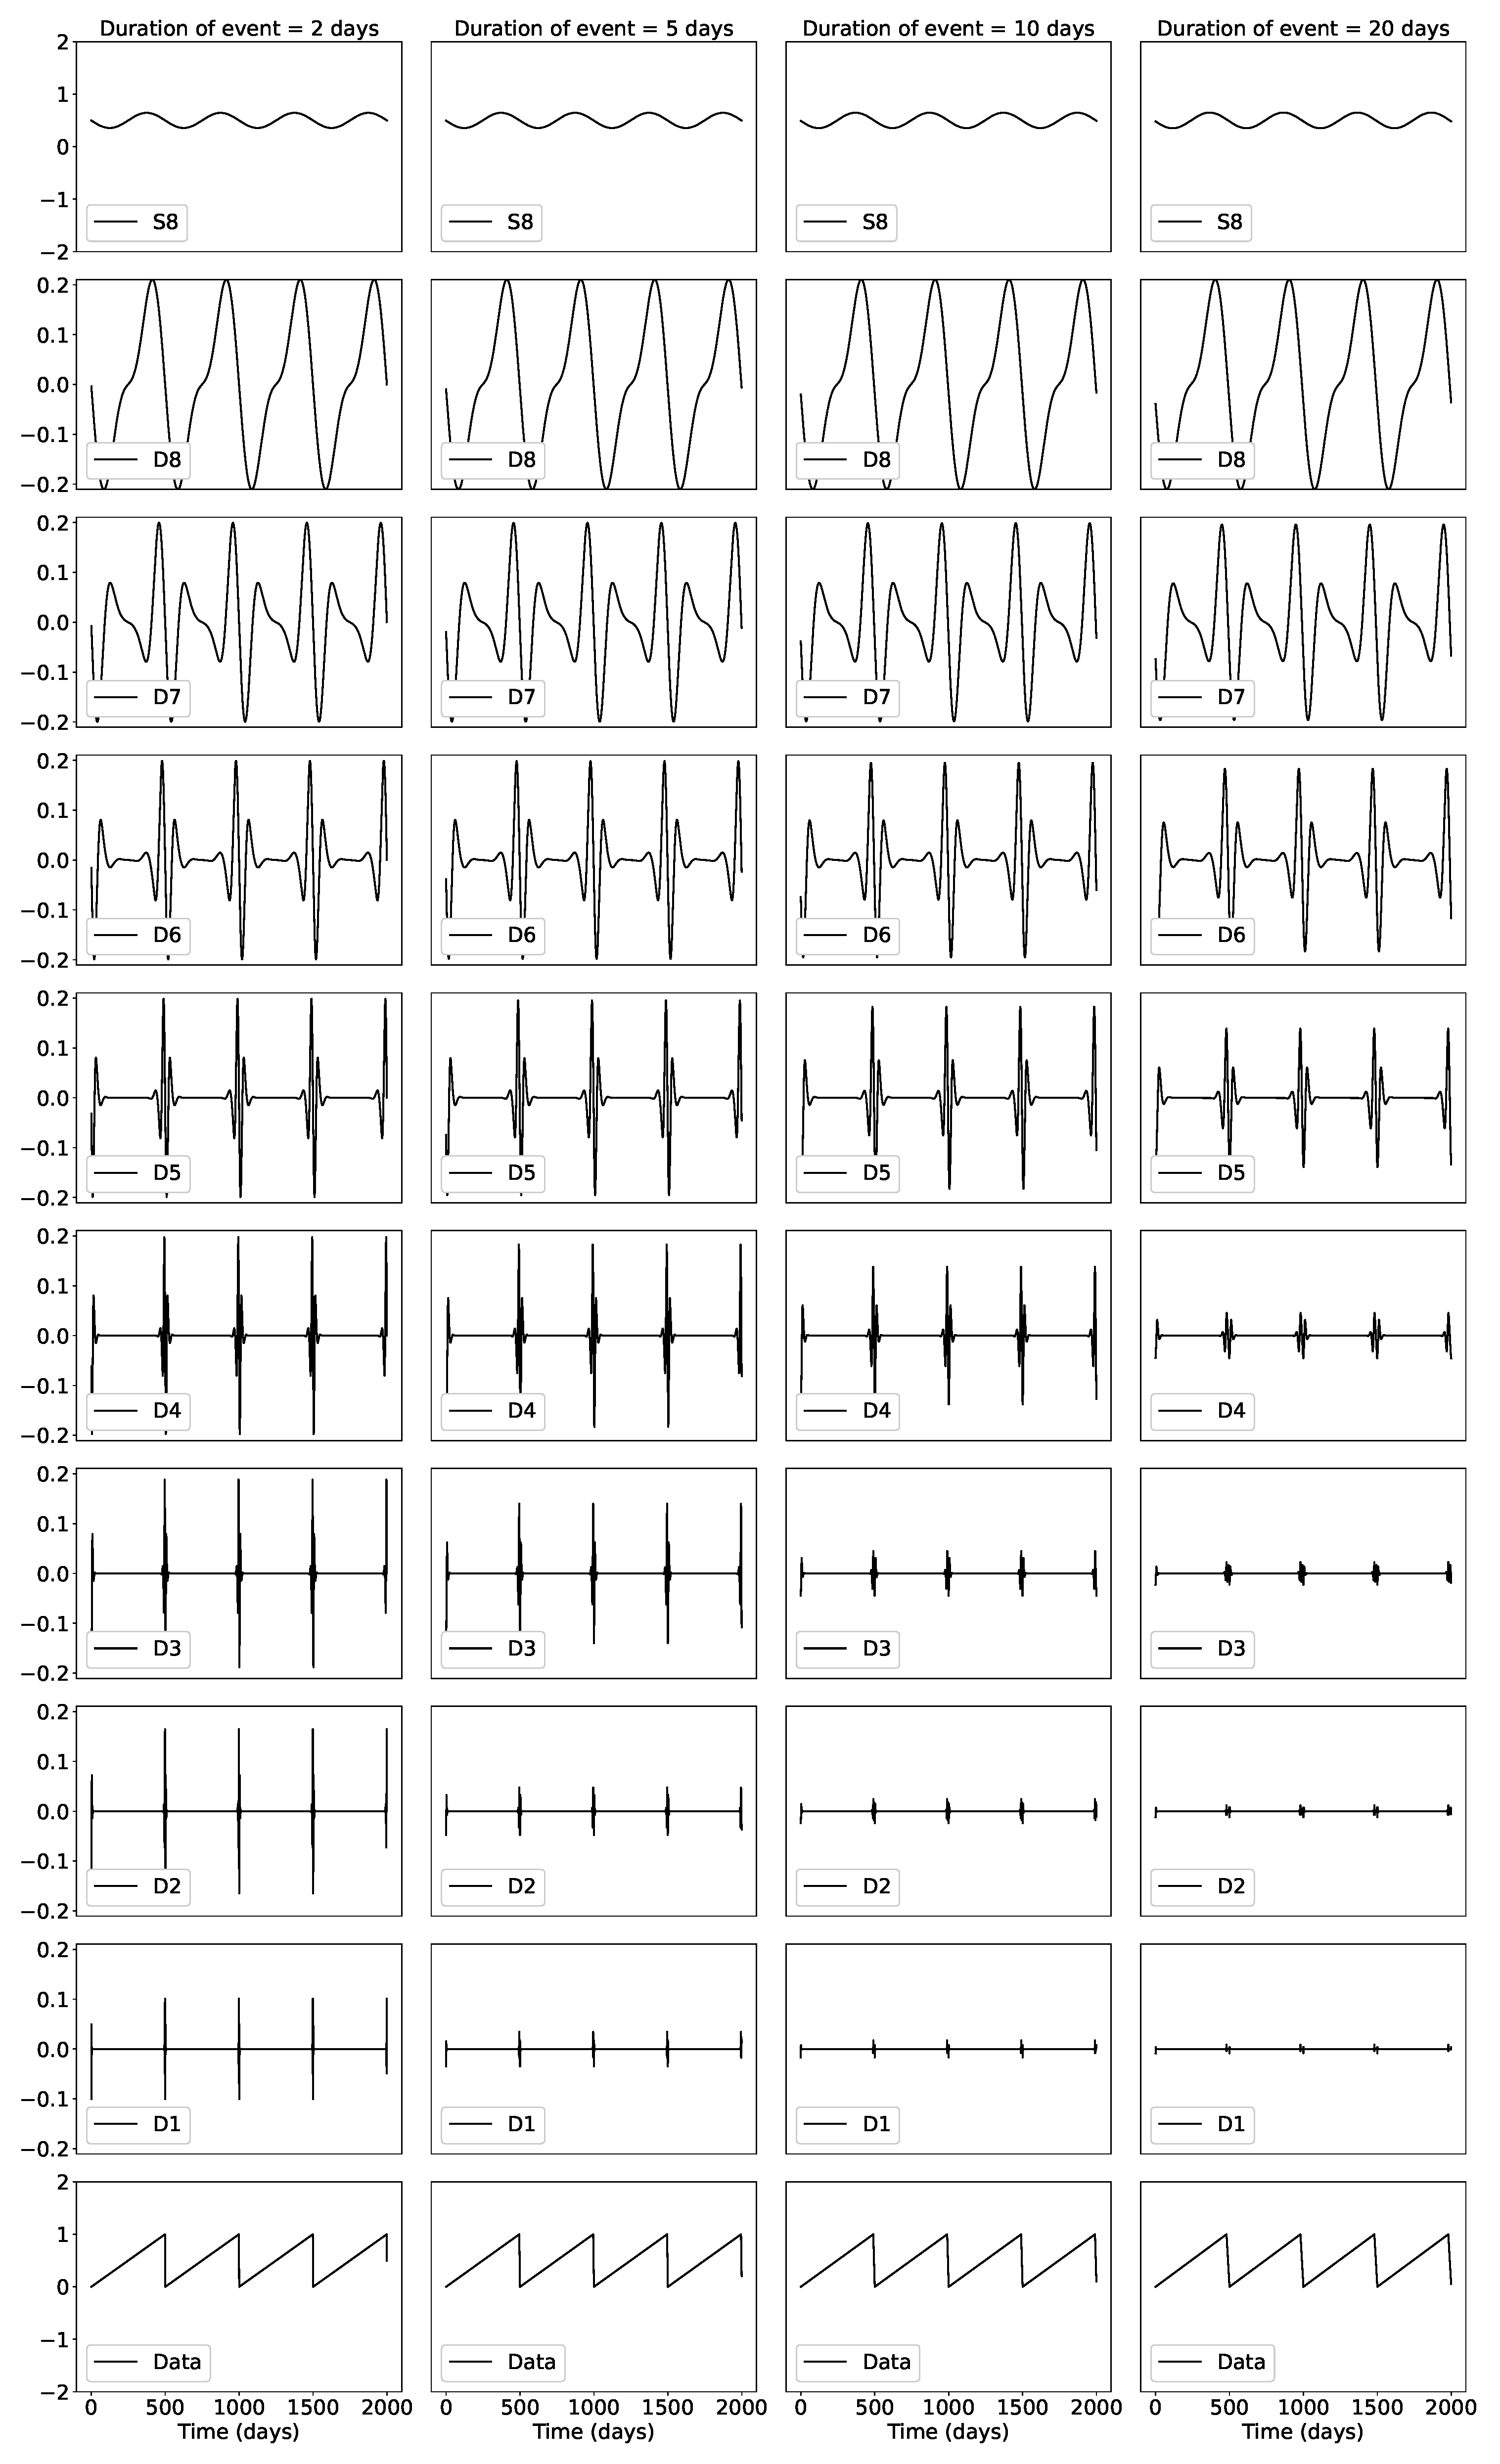
\includegraphics[width=10cm, trim={0cm 0cm 0cm 0cm},clip]{figures/500_DS.eps}
\caption{Demonstration of a wavelet decomposition for a synthetic dataset. A synthetic time series is created (top row) with steps of period 500 days, and transient durations of 2 days (left), 5 days, 10 days, and 20 days (right). The resulting details and smooths are shown in increasing level. The amplitude of the synthetic time series is normalized to 1, and the details and smooths show the relative amplitude.}
\label{pngfiguresample}
\end{figure}

\begin{figure}
\noindent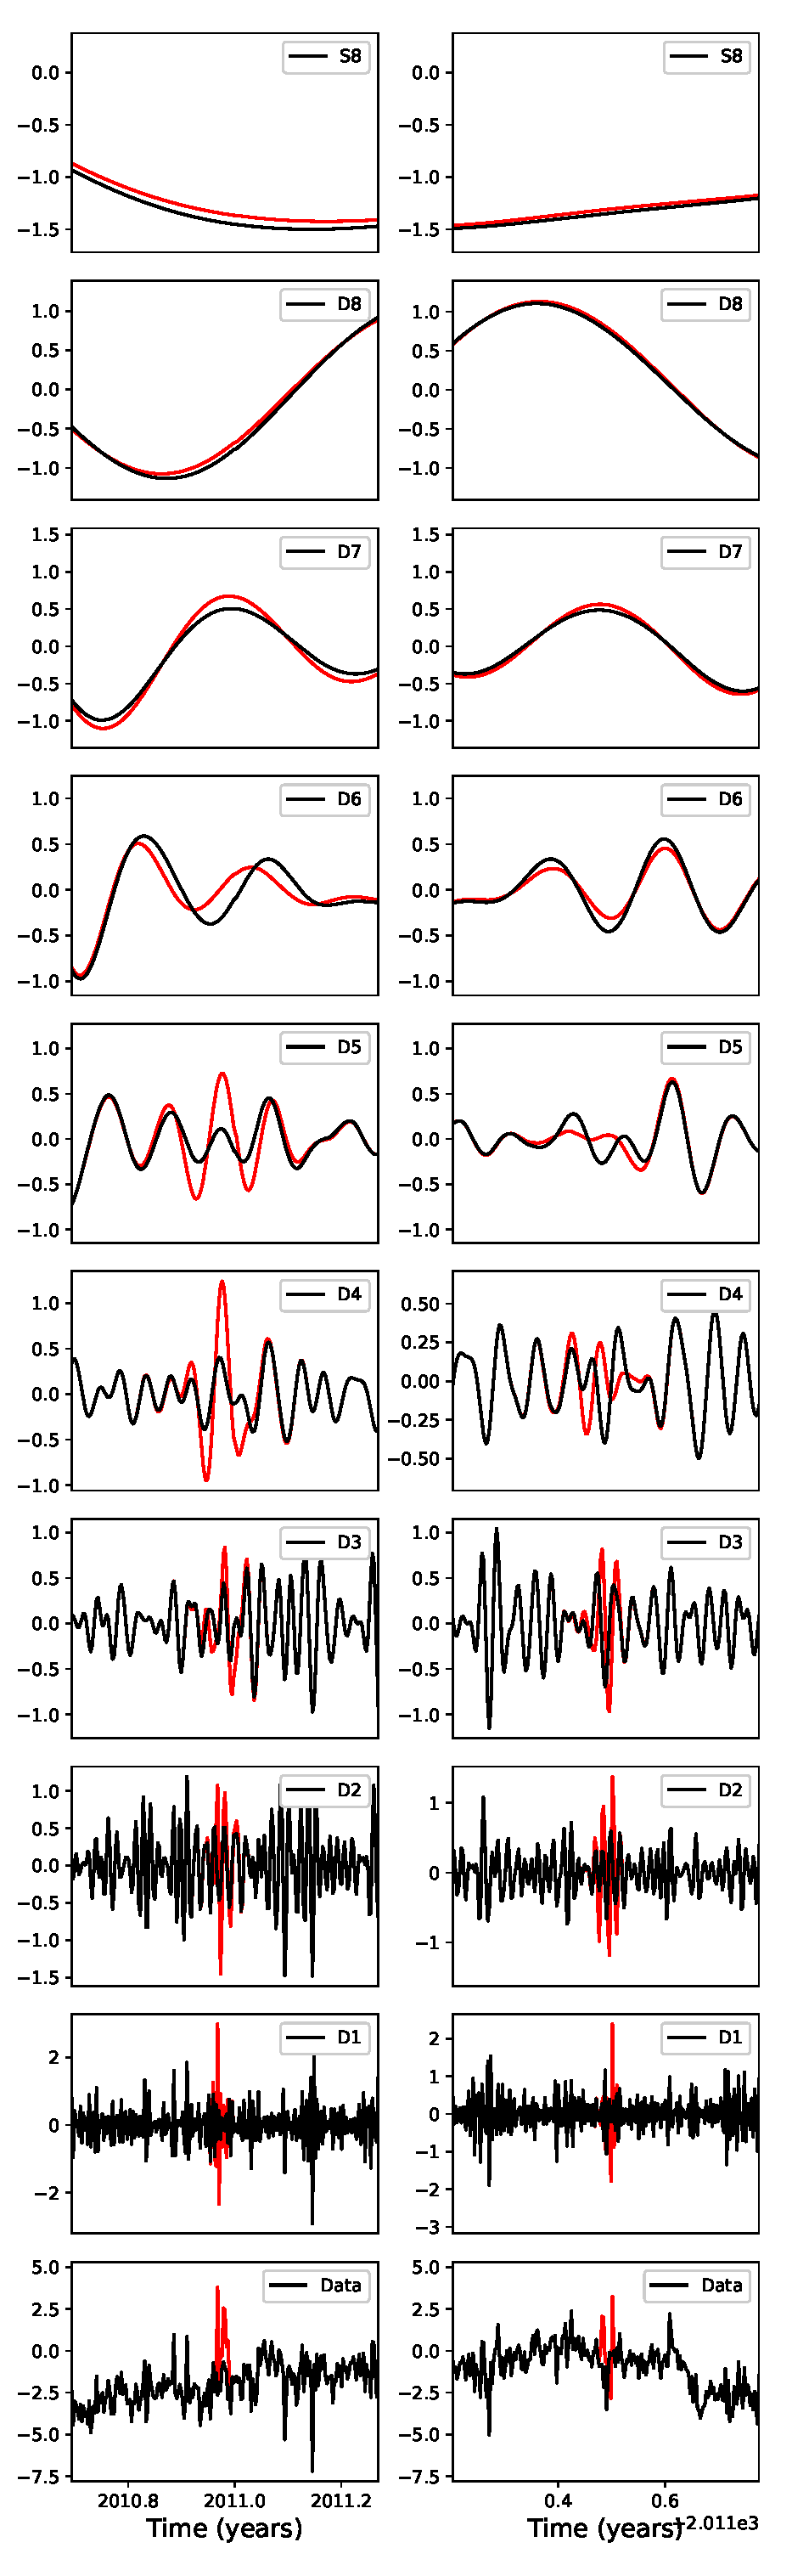
\includegraphics[width=5cm, trim={0cm 0cm 0cm 0cm},clip]{figures/DS_10.eps}
\caption{Top: Data from GPS station PGC5 without missing values (black) and with missing values replaced by the sum of a straight line and a Gaussian noise component (red) for two locations of the missing values (left and right). The corresponding ten details and smooths of the wavelet composition are shown in increasing levels for the original data (black) and for the missing values replaced by linear interpolation plus Gaussian noise (red).}
\label{pngfiguresample}
\end{figure}

\begin{figure}
\noindent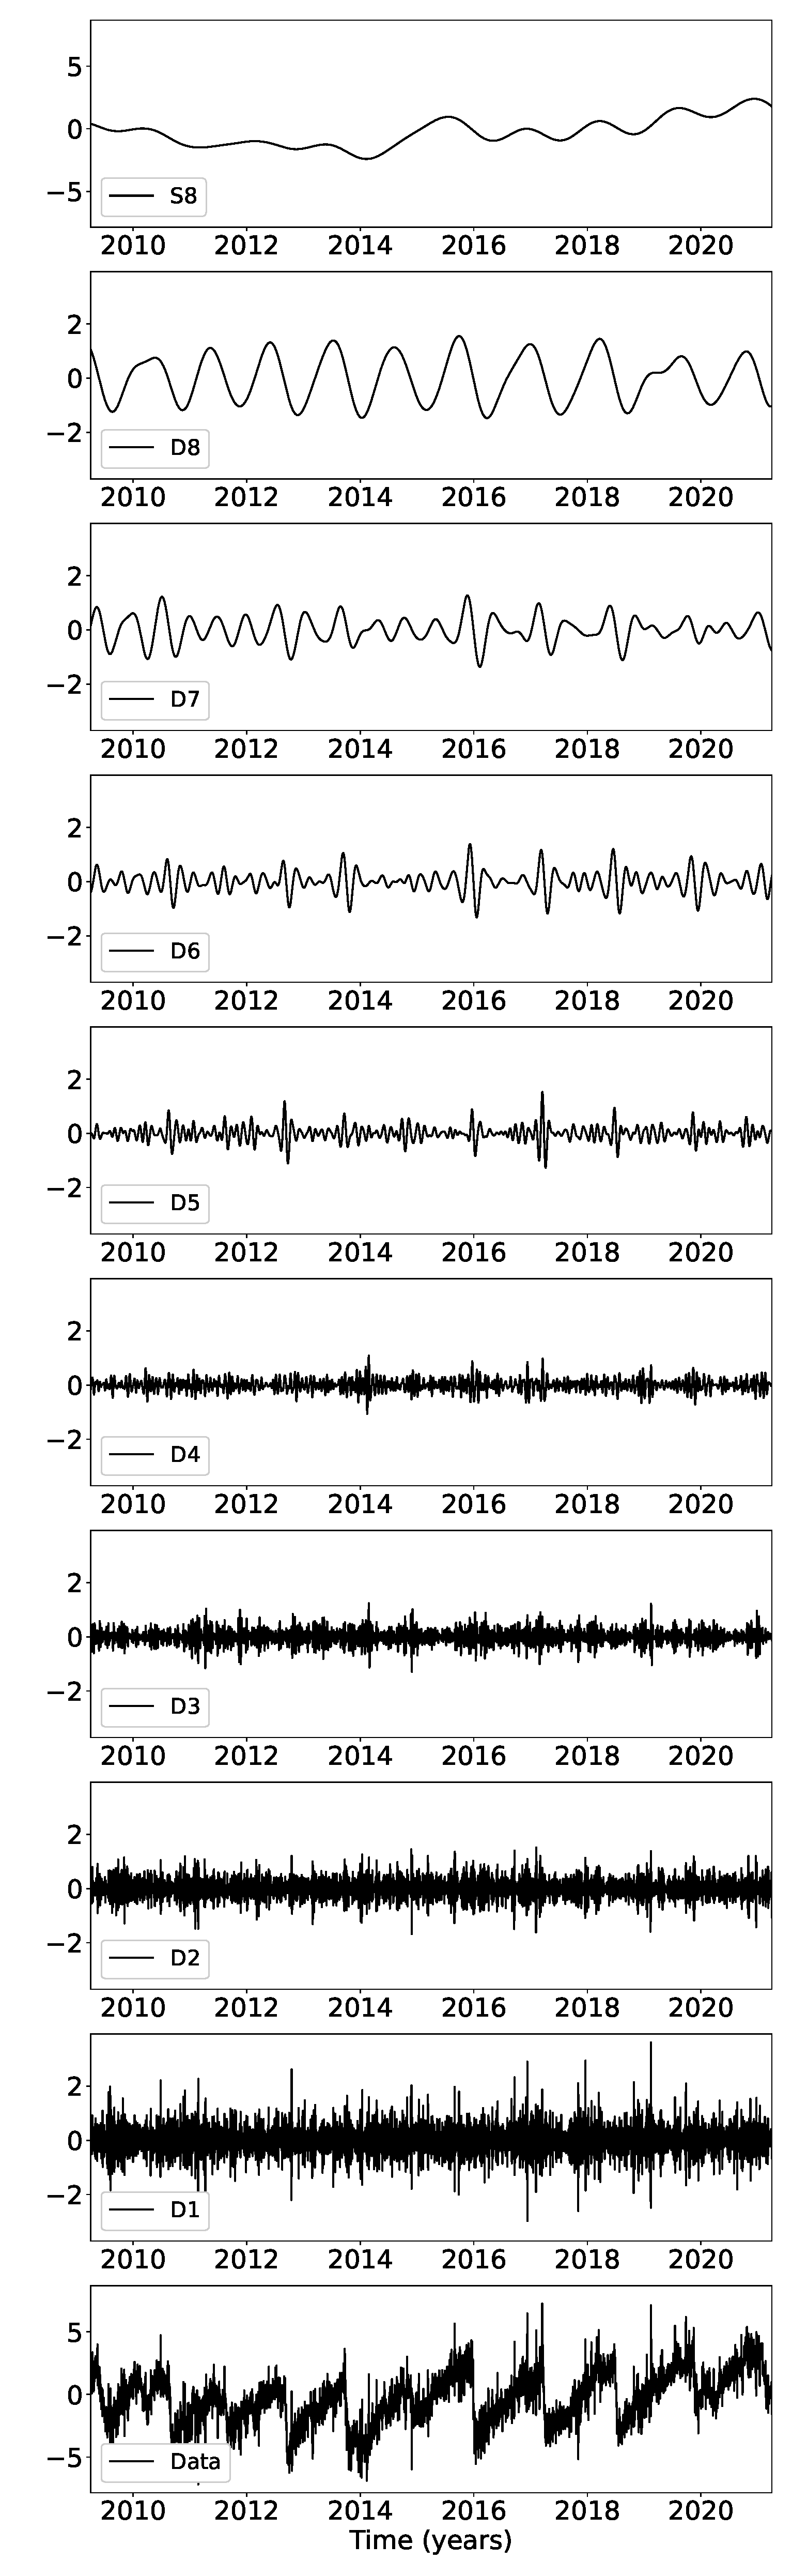
\includegraphics[width=5cm, trim={0cm 0cm 0cm 0cm},clip]{figures/cleaned_PGC5_lon.eps}
\caption{Top: Longitudinal displacement recorded at GPS station PGC5. The resulting details and smooth of the wavelet decomposition are shown in increasing level.}
\label{pngfiguresample}
\end{figure}

\begin{figure}
\noindent\includegraphics[width=\textwidth, trim={0cm 0cm 0cm 0cm},clip]{figures/map_GPS_stations.eps}
\caption{GPS stations used in this study (black triangles). The black line represents the 40 km depth contour of the plate boundary model by ~\citet{PRE_2003}. The red triangles are the locations where we stack the GPS data. The small grey dots are all the tremor locations from the PNSN catalog.}
\label{pngfiguresample}
\end{figure}

\begin{figure}
\noindent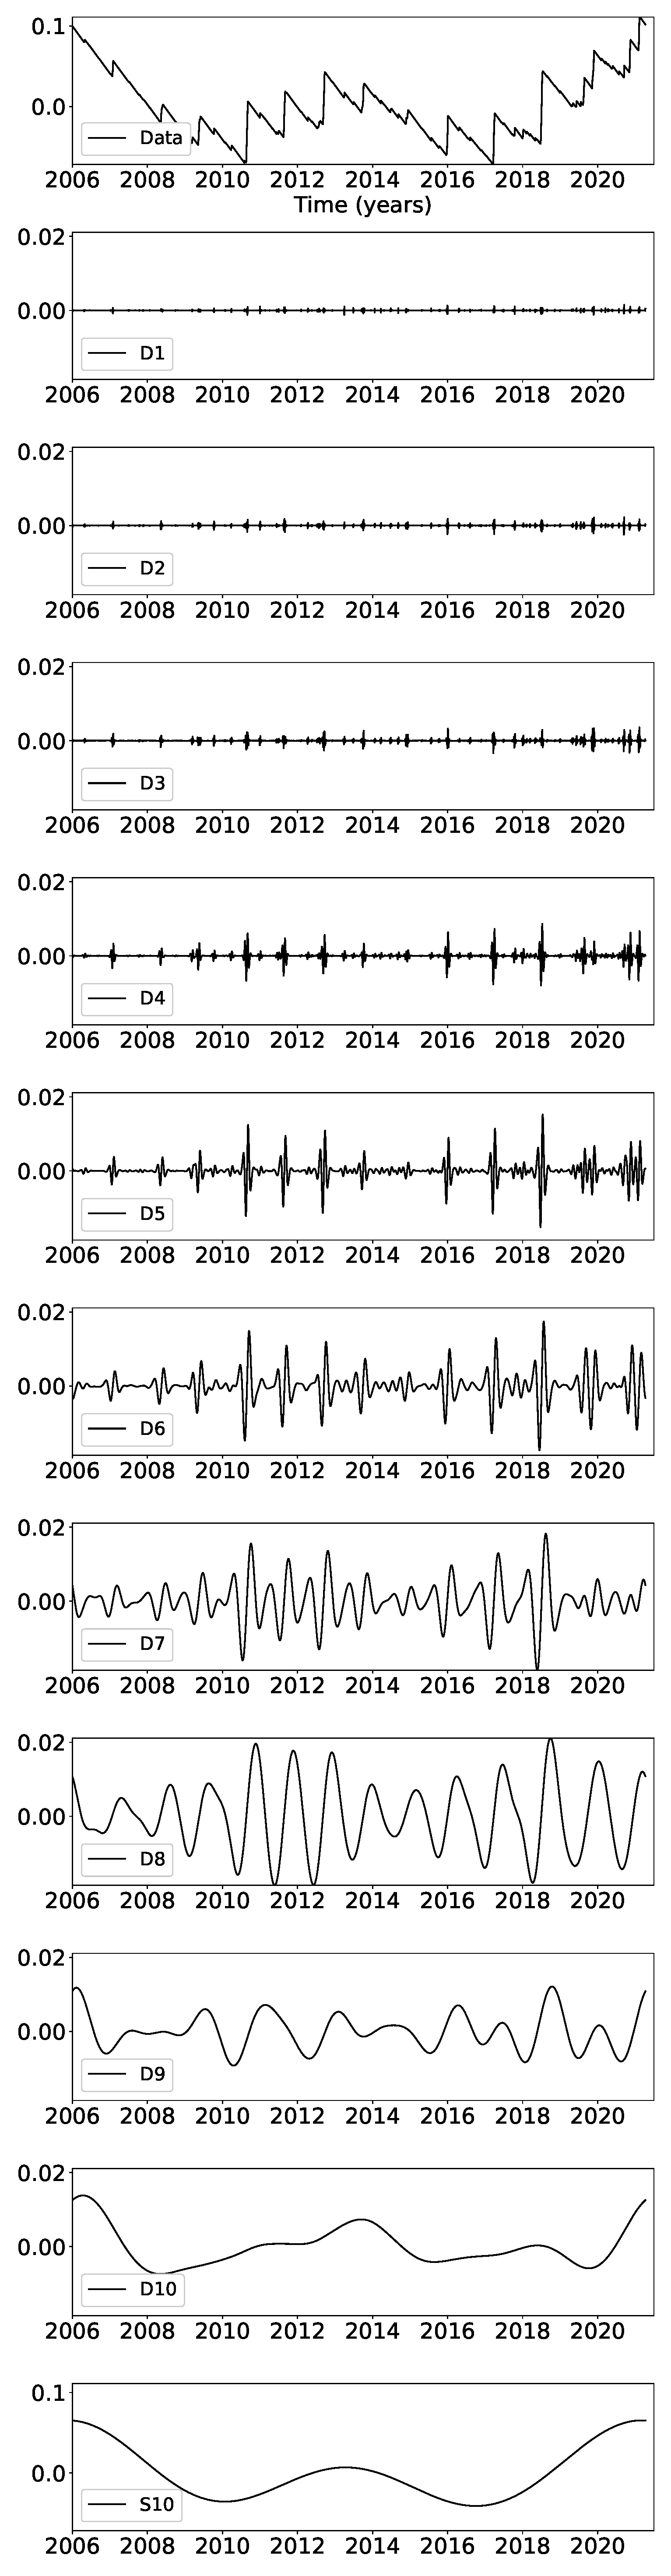
\includegraphics[width=5cm, trim={0cm 0cm 0cm 0cm},clip]{figures/tremor_13.eps}
\caption{Details and smooth of the wavelet decomposition of the detrended cumulative tremor count around the third northernmost red triangles on Figure 3 (latitude 48.5).}
\label{pngfiguresample}
\end{figure}

\begin{figure}
\noindent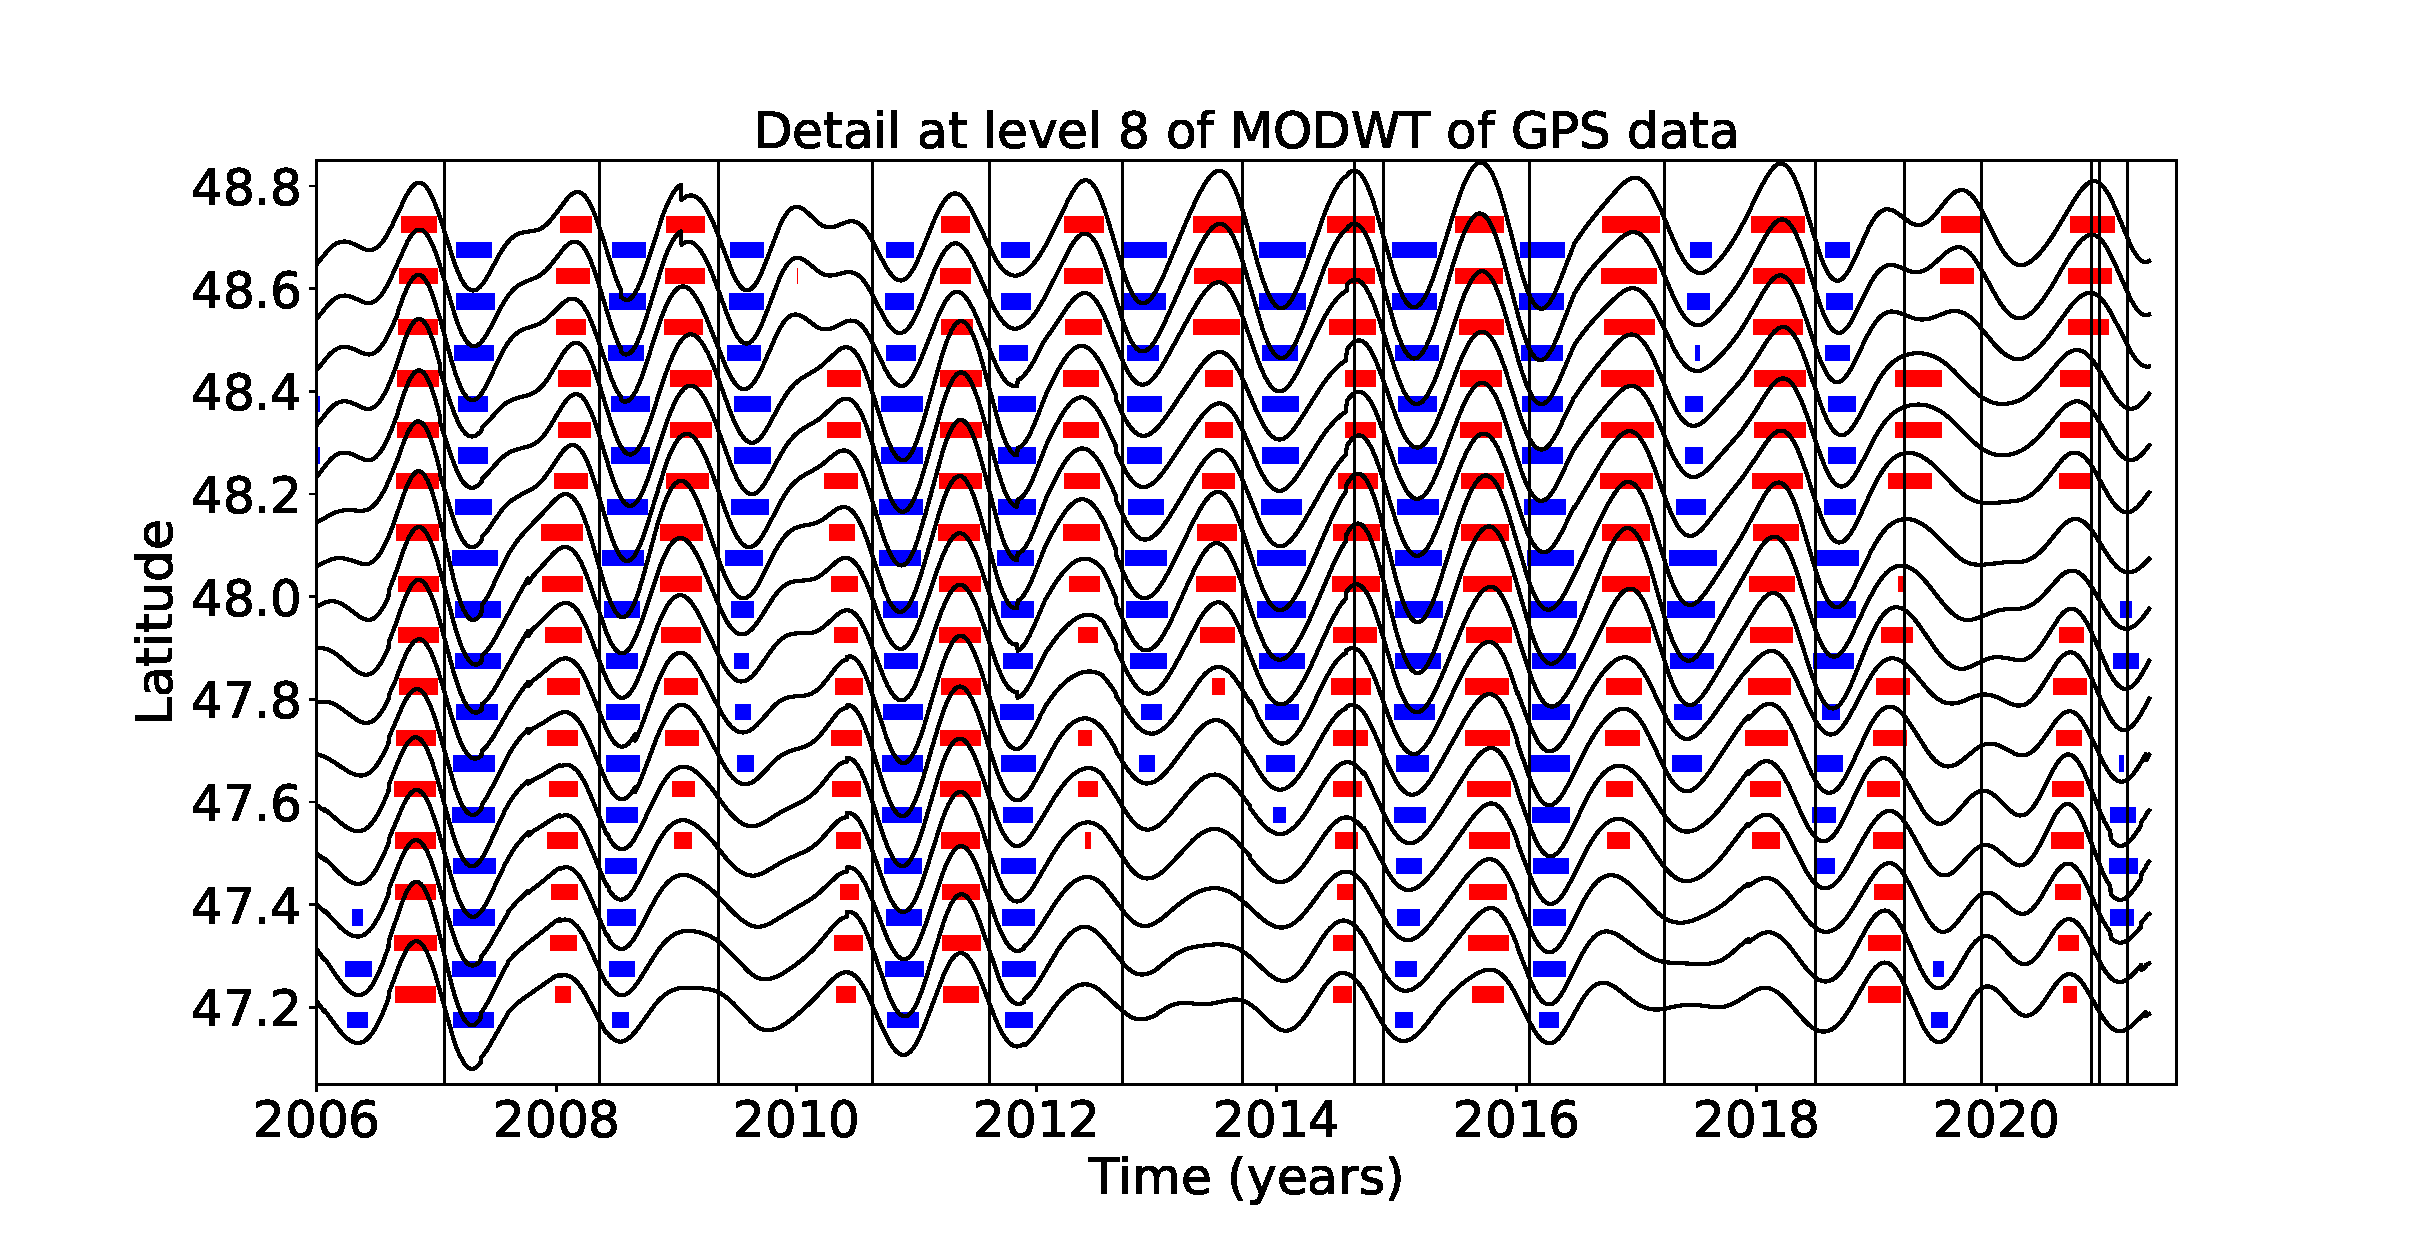
\includegraphics[width=\textwidth, trim={0cm 0cm 0cm 0cm},clip]{figures/GPS_longer_detail_8.eps}

\noindent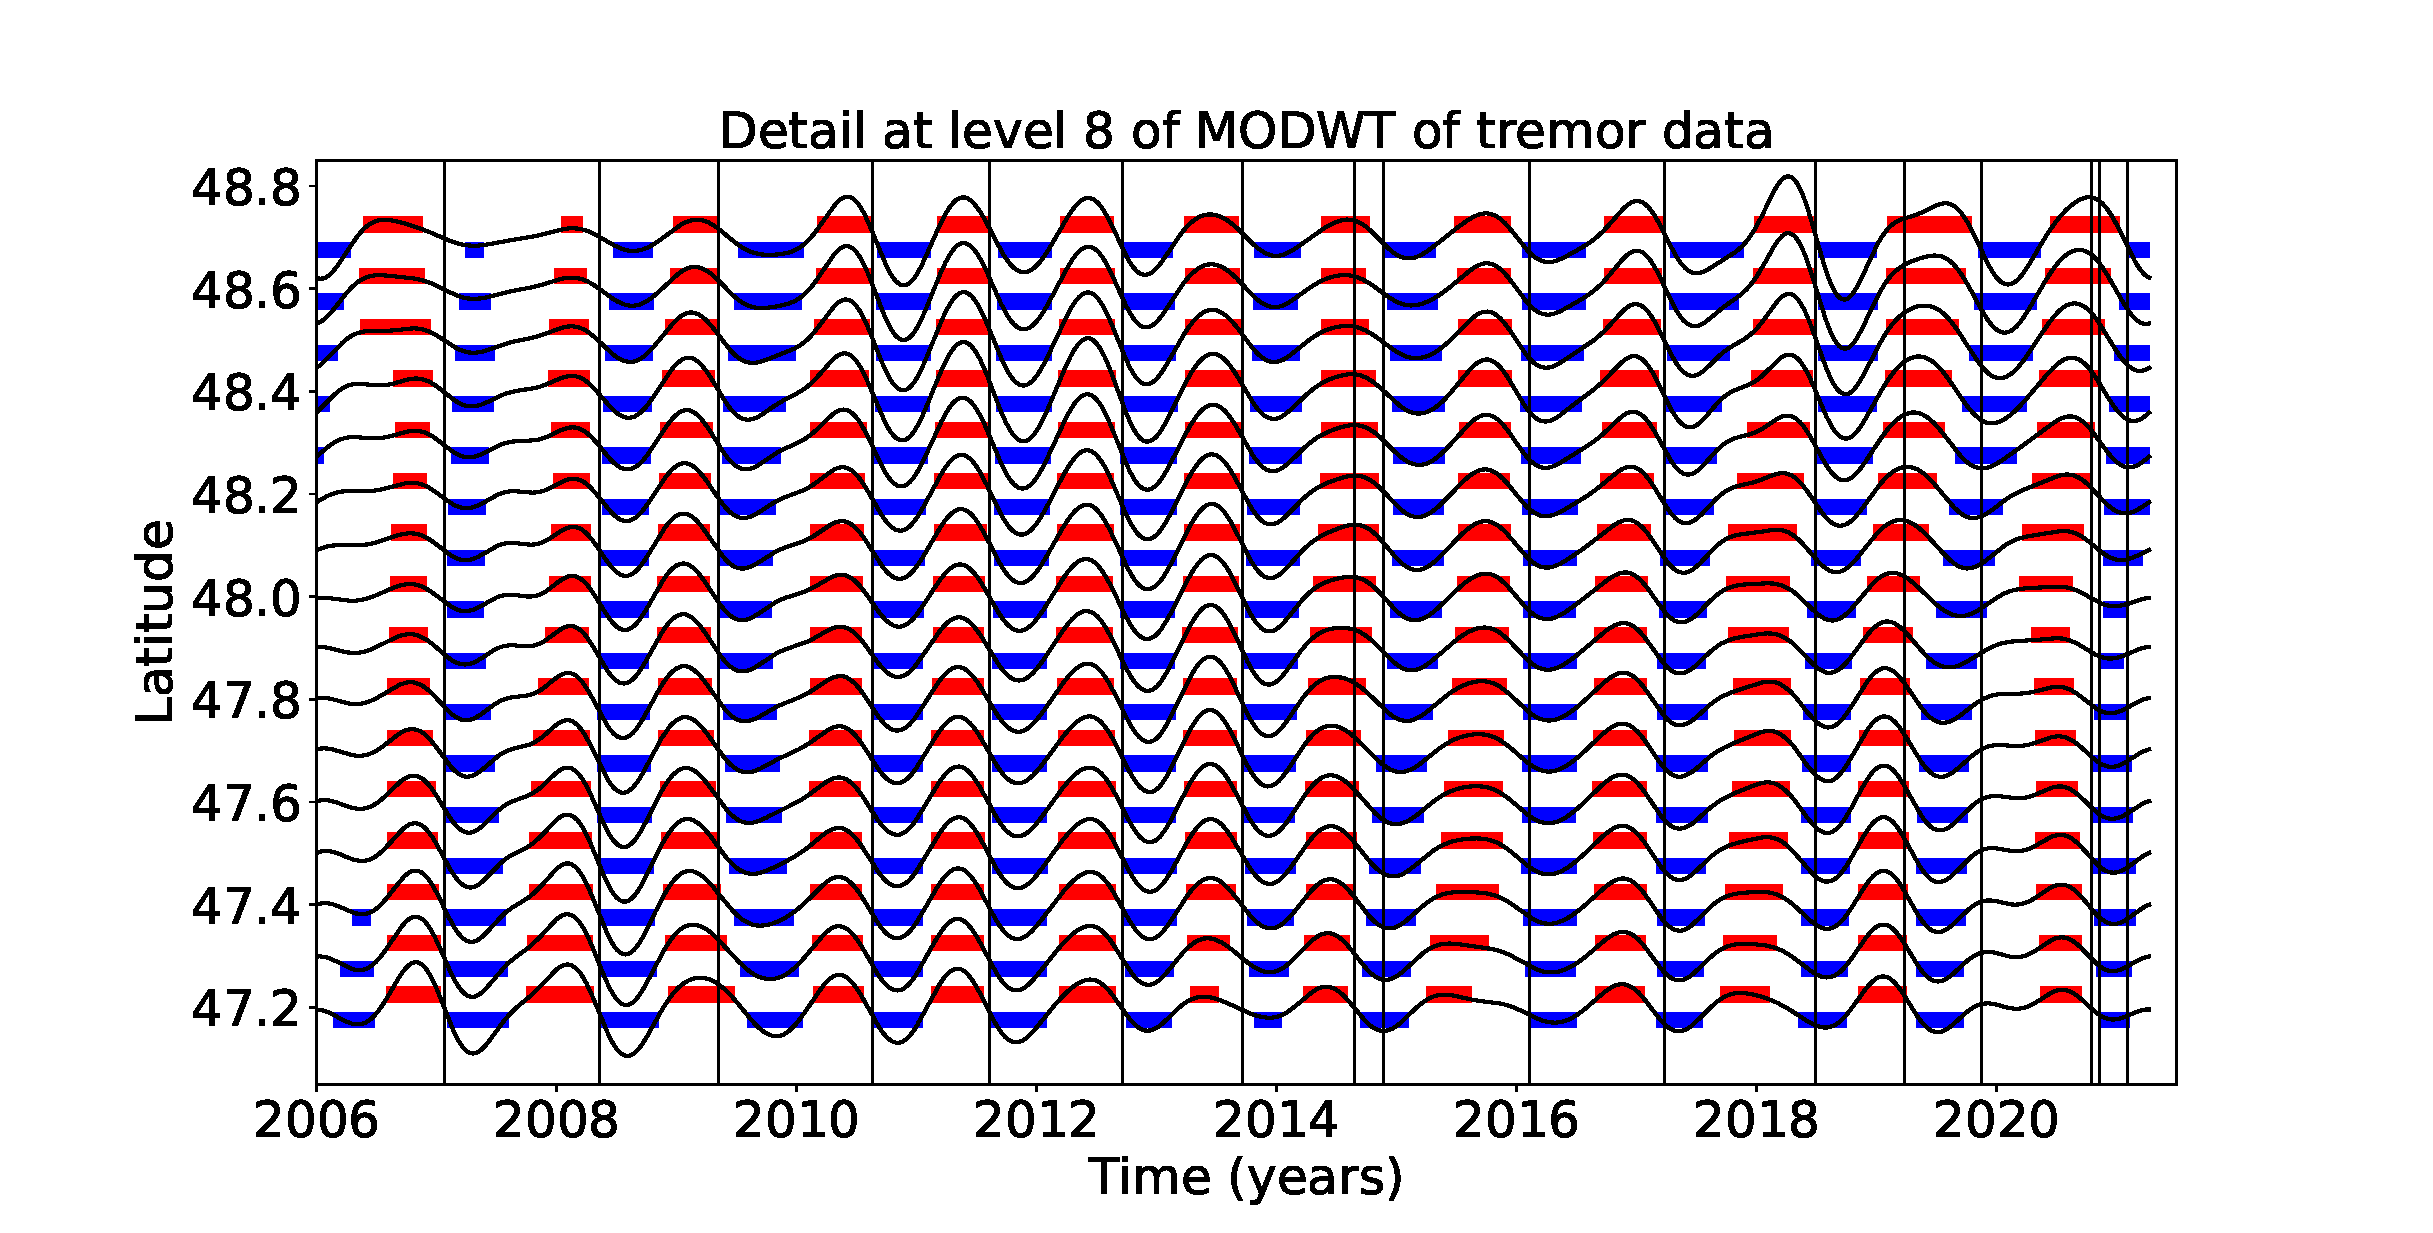
\includegraphics[width=\textwidth, trim={0cm 0cm 0cm 0cm},clip]{figures/tremor_longer_detail_8.eps}
\caption{Top: Stacked 8th level details of the wavelet decomposition of the displacement over all the GPS stations located in a 50 km radius of a given point, for the 16 red triangles indicated in Figure 3. Bottom: 8th level detail multiplied by -1 of the cumulative tremor count in a 50 km radius of a given point for the same 16 locations. The black lines represent the timings of the ETS events from Table 1. We mark by a red rectangle every time where the amplitude is higher than a threshold of 0.4 (for the GPS) or 0.003 (for the tremor). We mark by a blue rectangle every time where the amplitude is lower than minus the threshold.}
\label{pngfiguresample}
\end{figure}

\begin{figure}
\noindent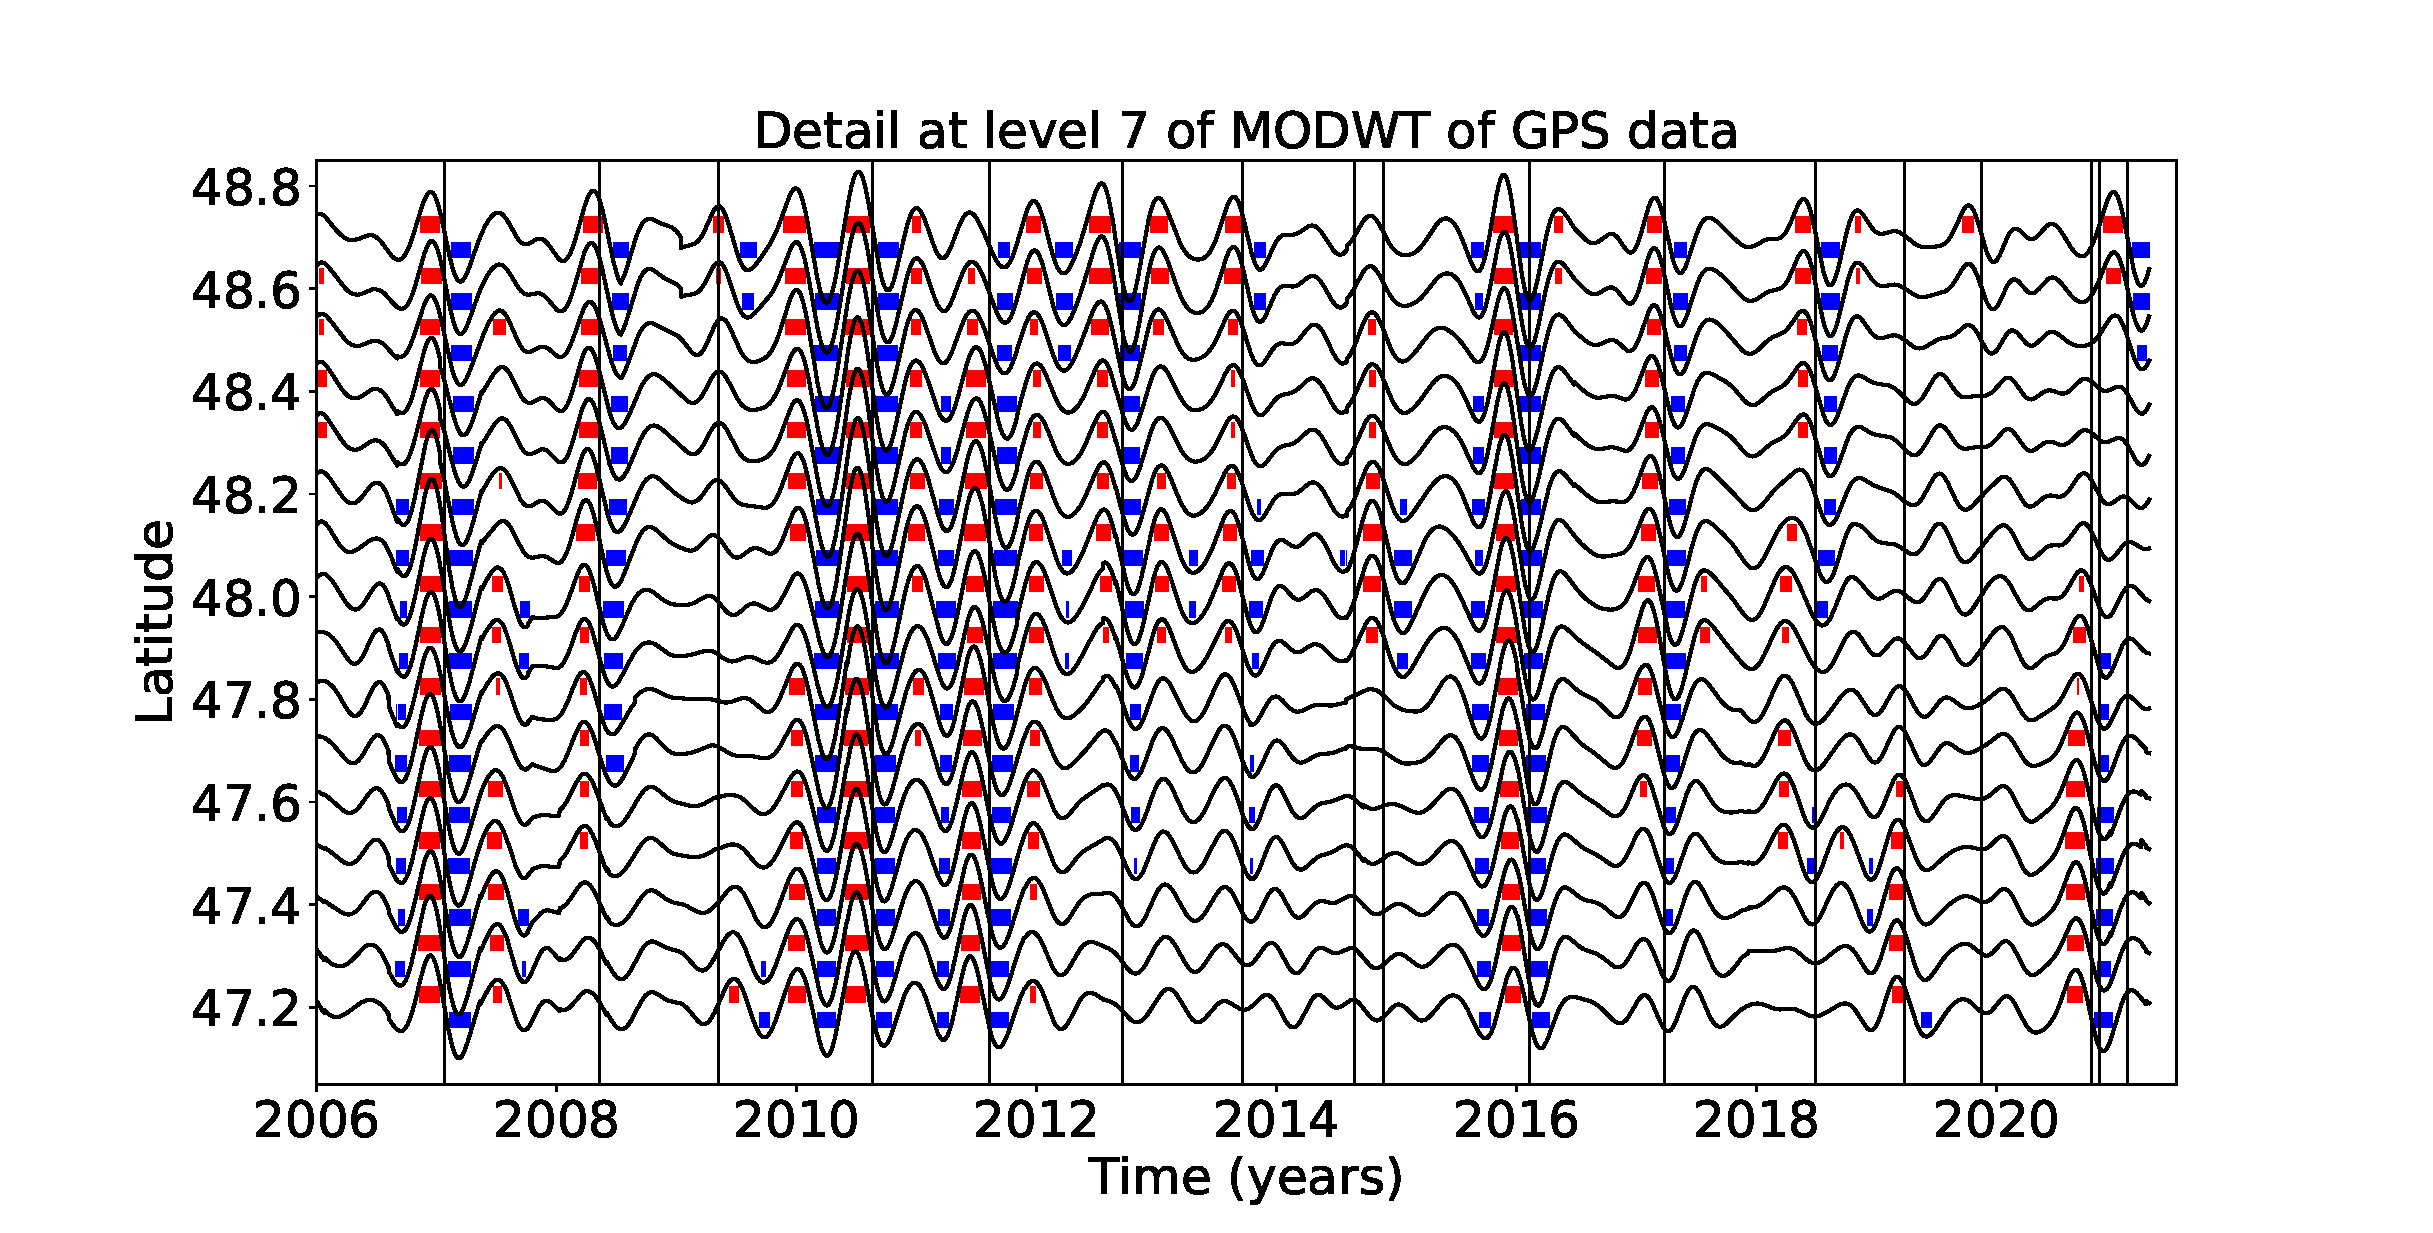
\includegraphics[width=\textwidth, trim={0cm 0cm 0cm 0cm},clip]{figures/GPS_longer_detail_7.eps}

\noindent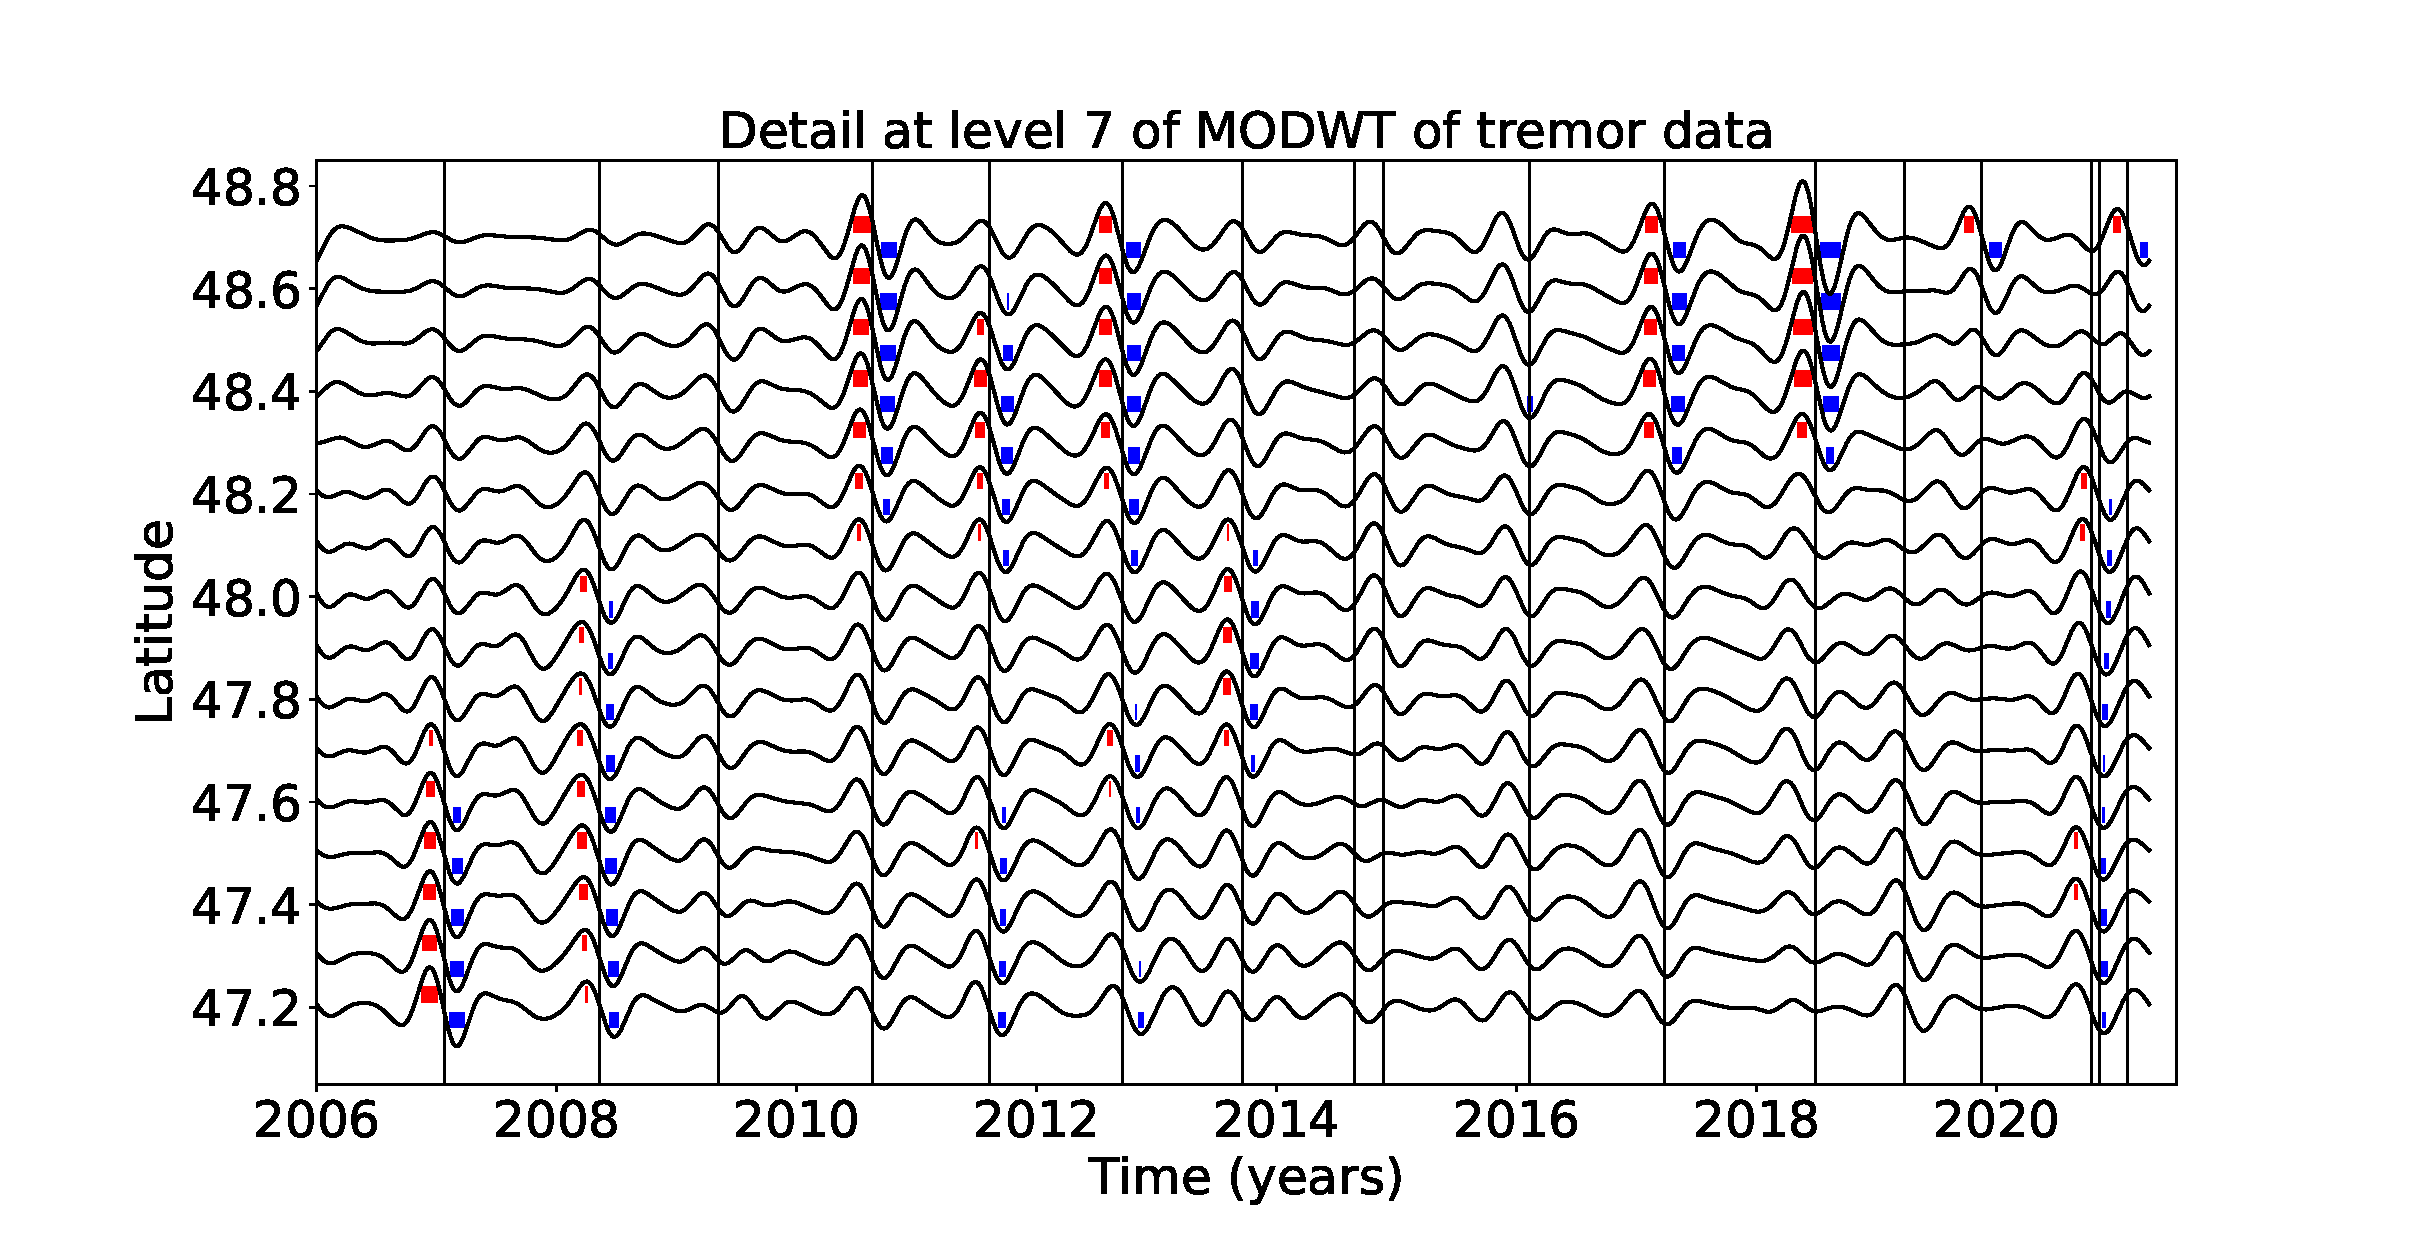
\includegraphics[width=\textwidth, trim={0cm 0cm 0cm 0cm},clip]{figures/tremor_longer_detail_7.eps}
\caption{Same as Figure 6 but for the 7th level detail. The thresholds are 0.5 (for the GPS) and 0.01 (for the tremor).}
\label{pngfiguresample}
\end{figure}

\begin{figure}
\noindent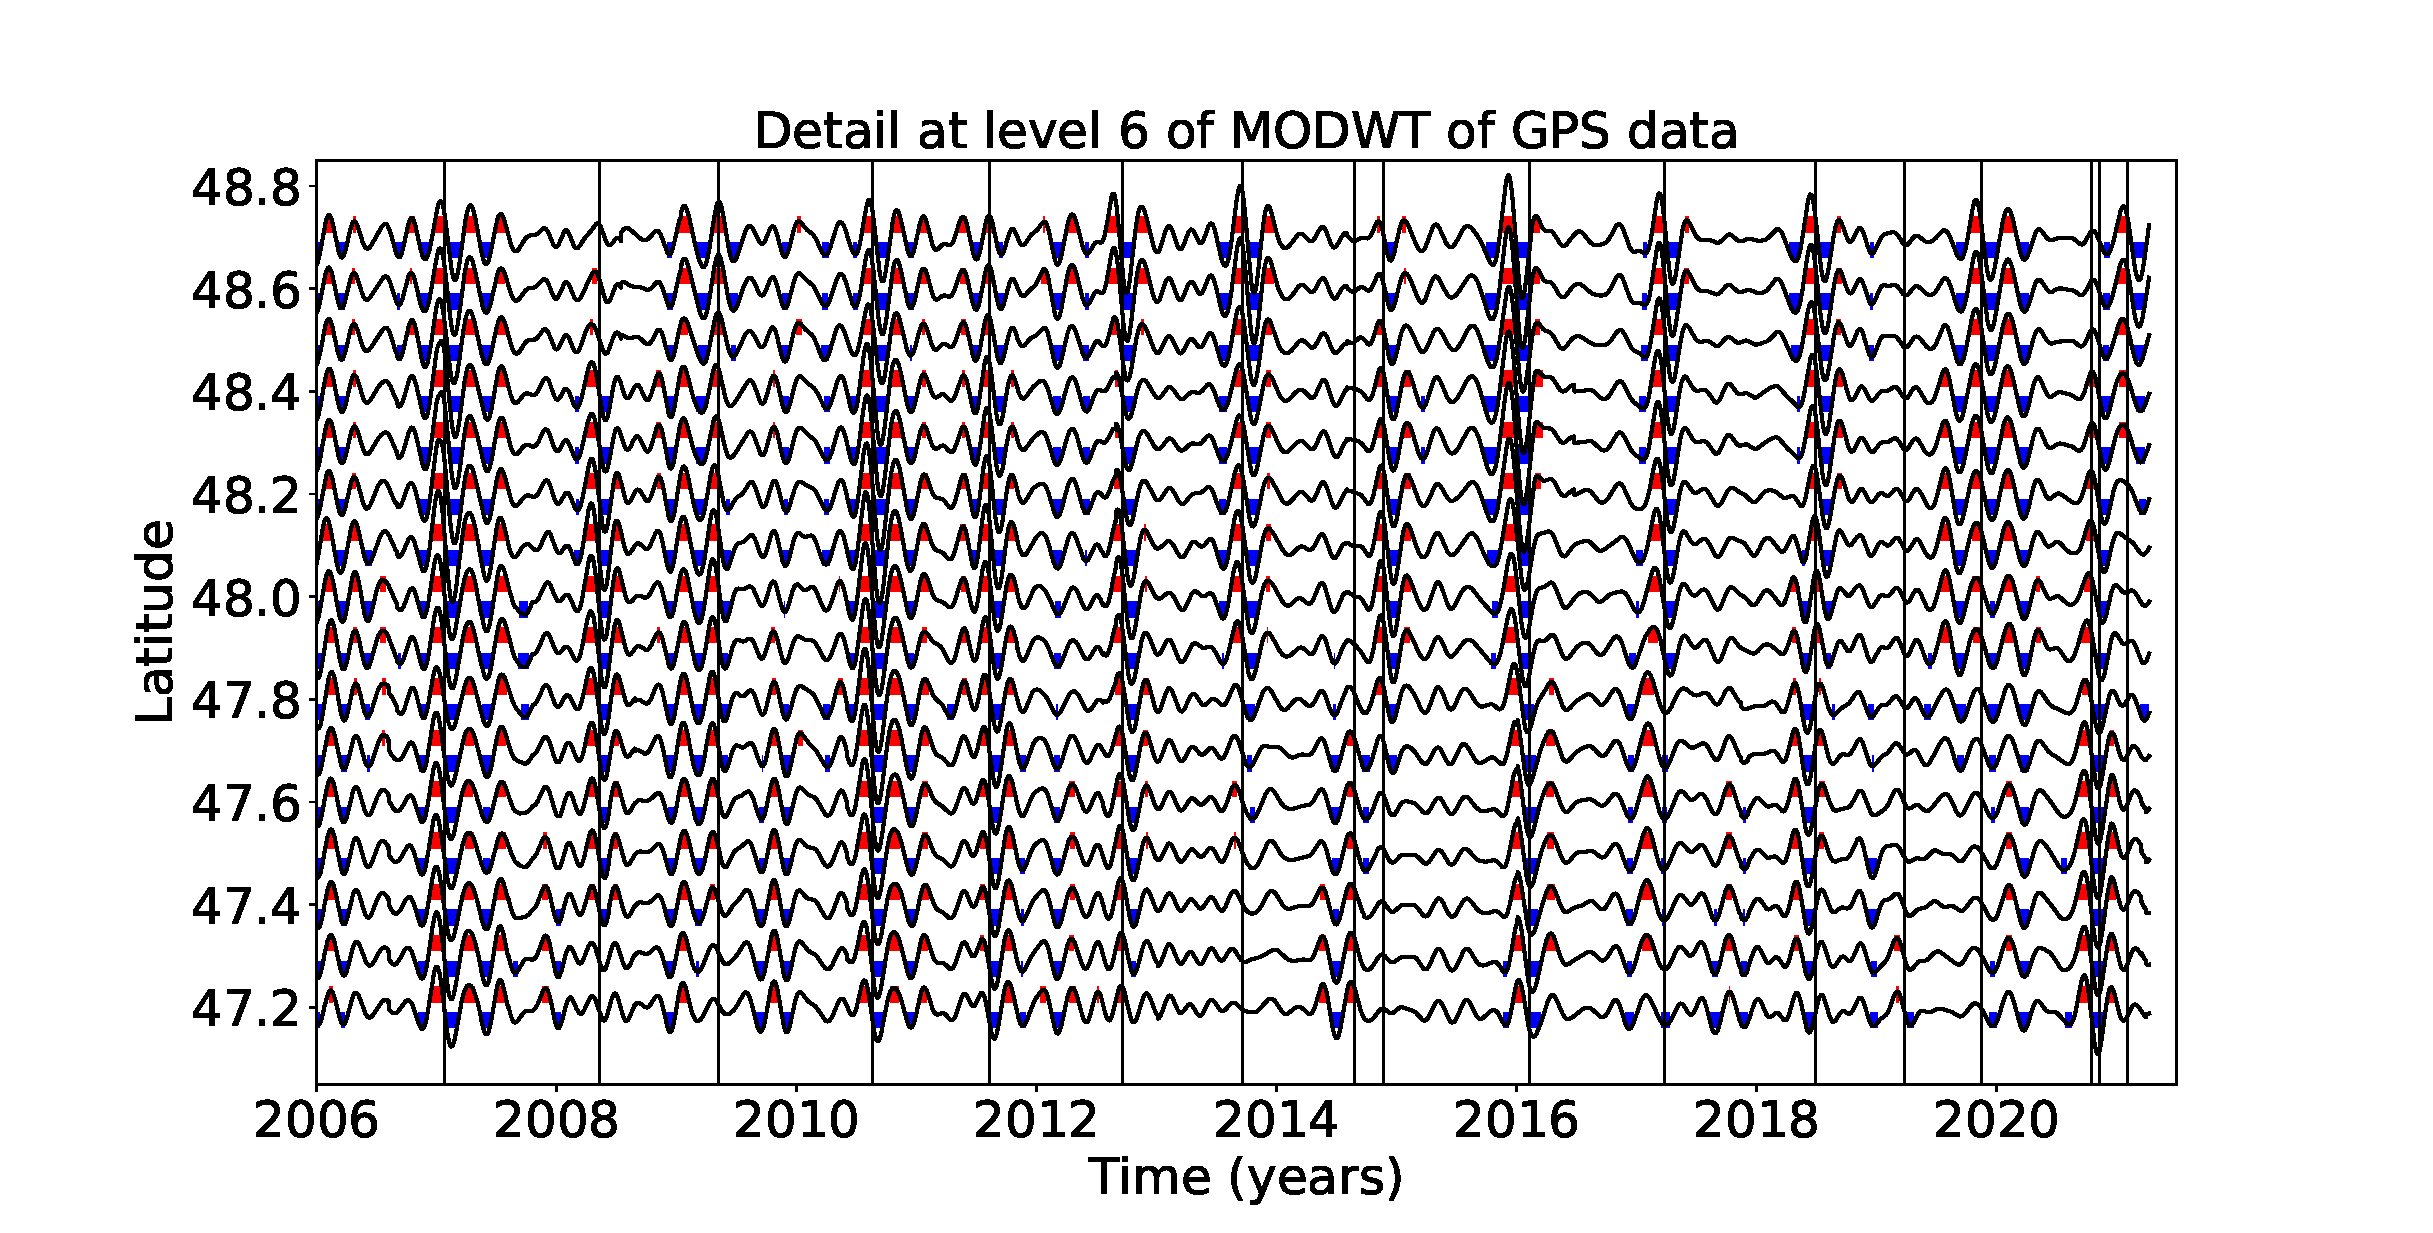
\includegraphics[width=\textwidth, trim={0cm 0cm 0cm 0cm},clip]{figures/GPS_longer_detail_6.eps}

\noindent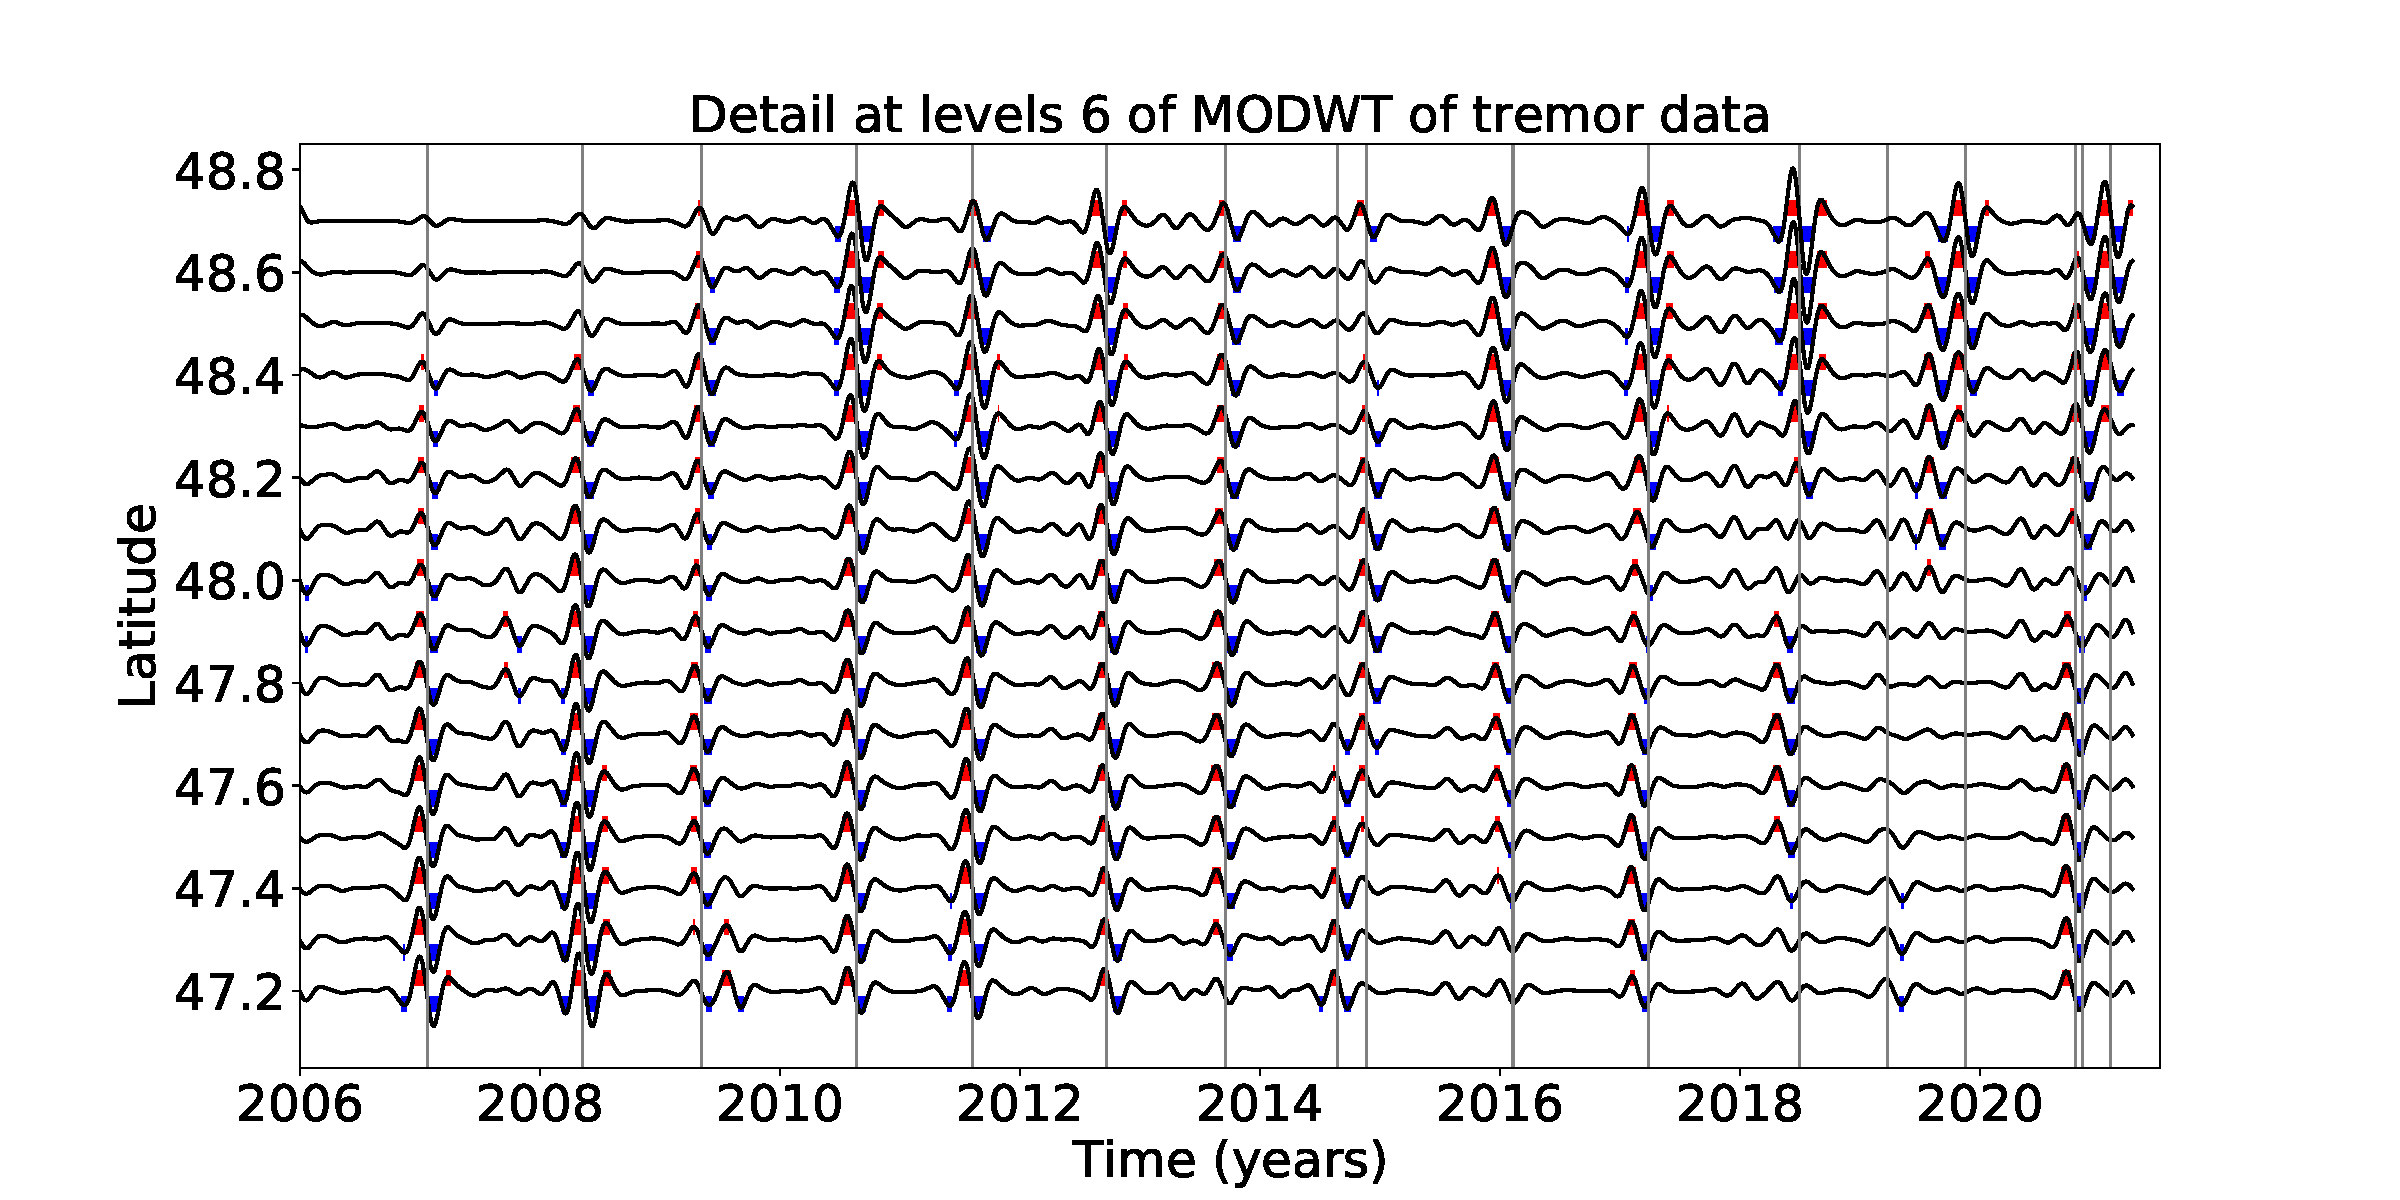
\includegraphics[width=\textwidth, trim={0cm 0cm 0cm 0cm},clip]{figures/tremor_longer_detail_6.pdf}
\caption{Same as Figure 6 but for the 6th level detail. The thresholds are 0.3 (for the GPS) and 0.009 (for the tremor).}
\label{pngfiguresample}
\end{figure}

\begin{figure}
\noindent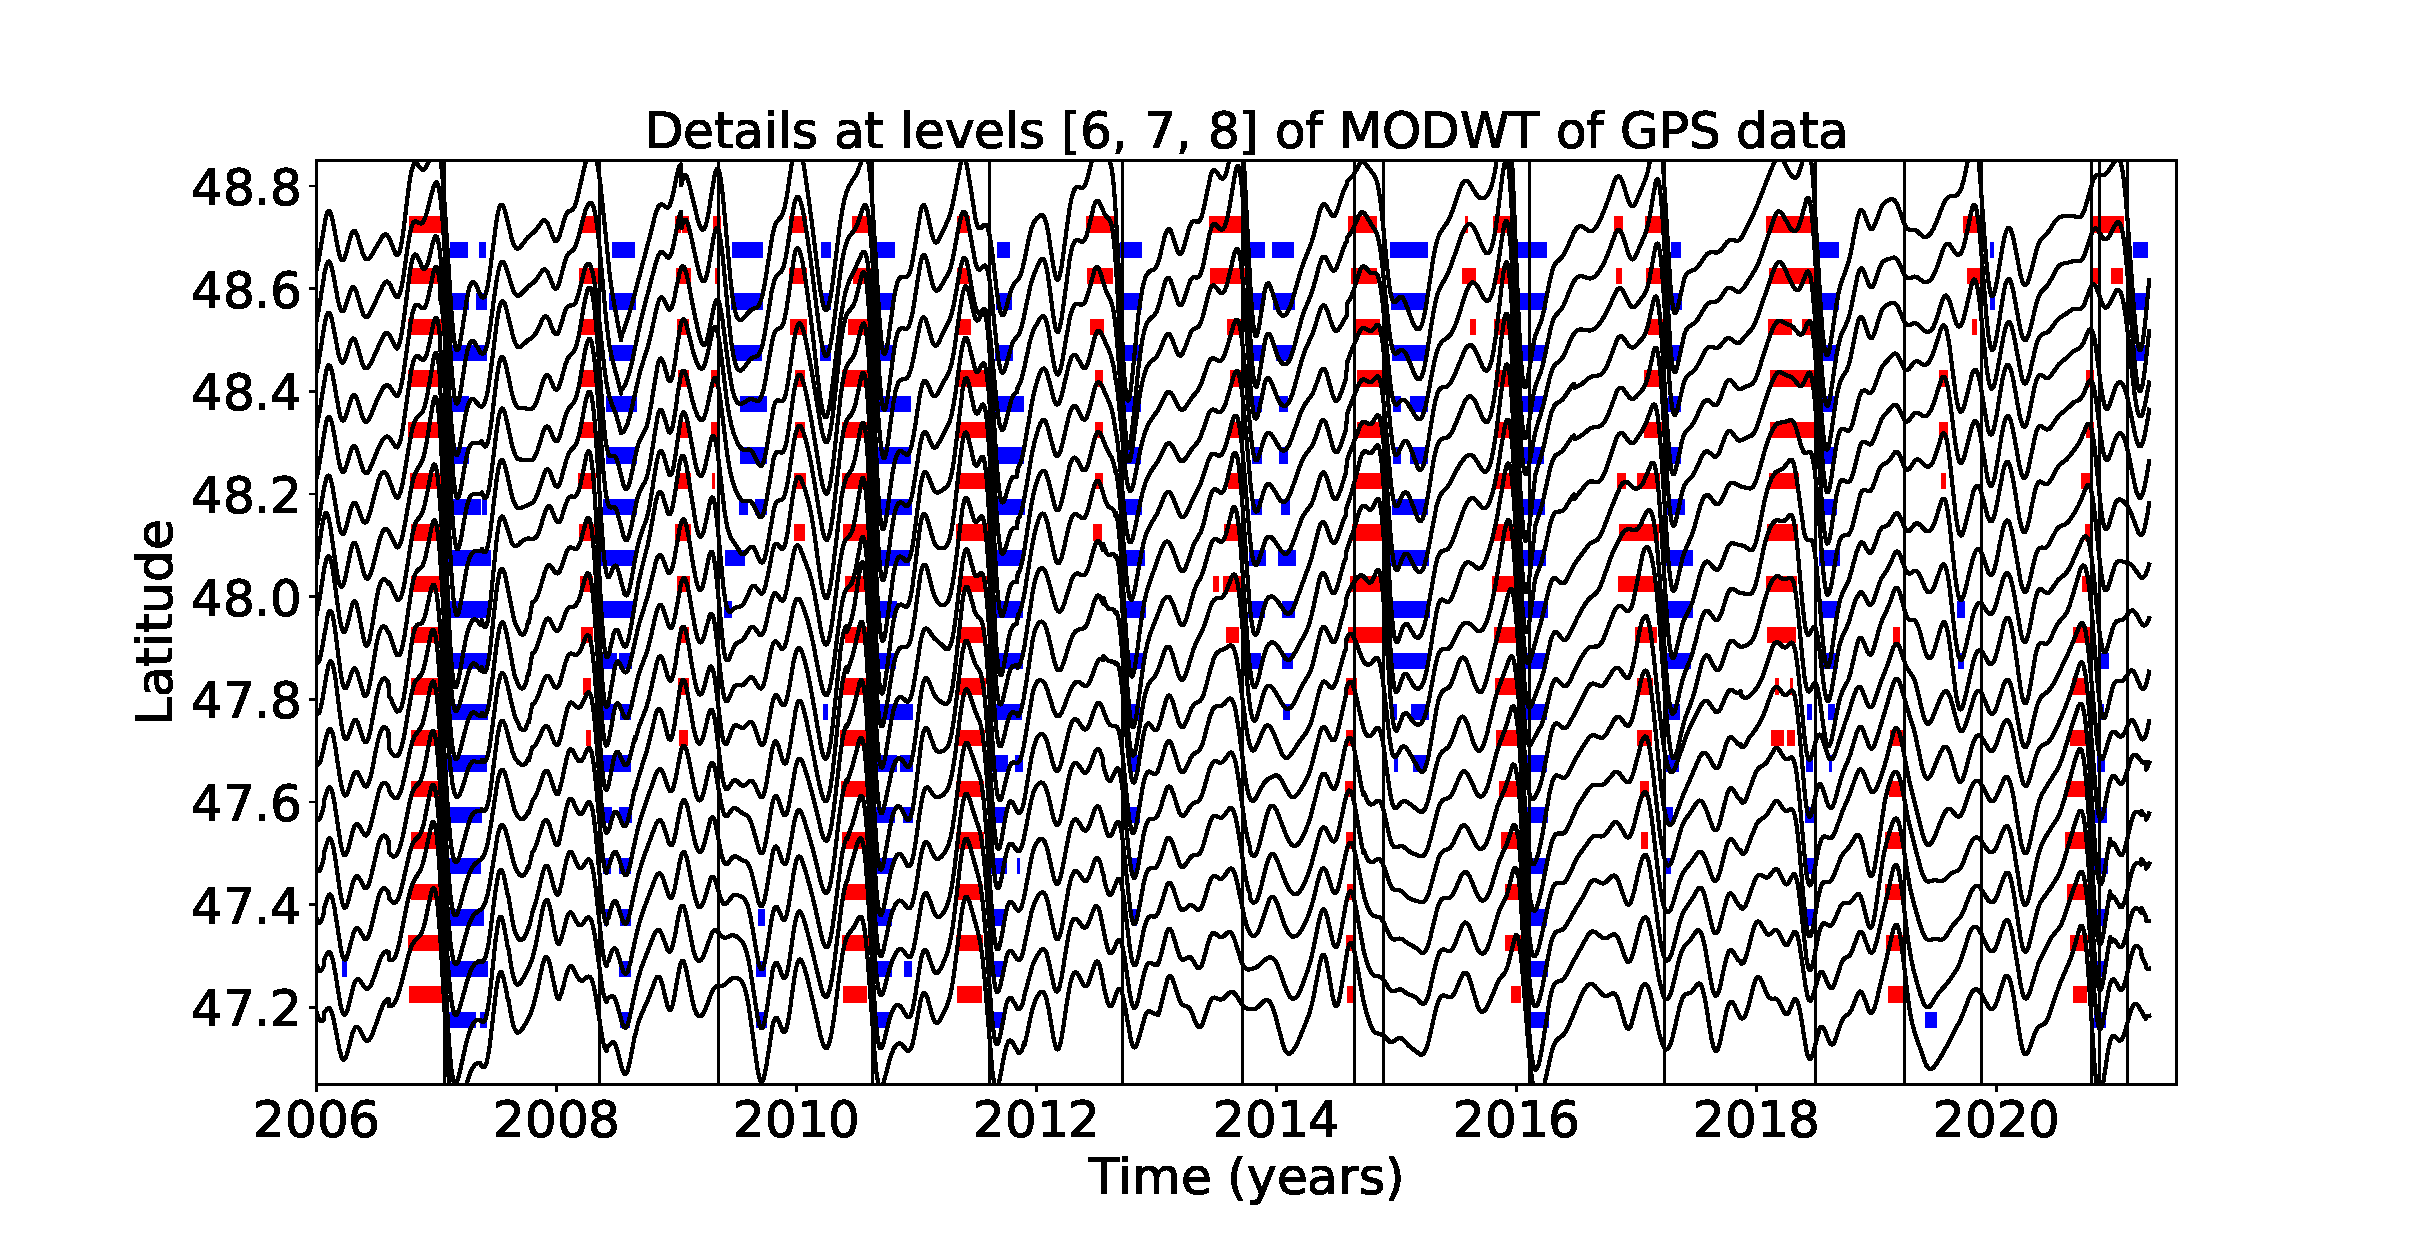
\includegraphics[width=\textwidth, trim={0cm 0cm 0cm 0cm},clip]{figures/GPS_longer_detail_6-7-8.eps}

\noindent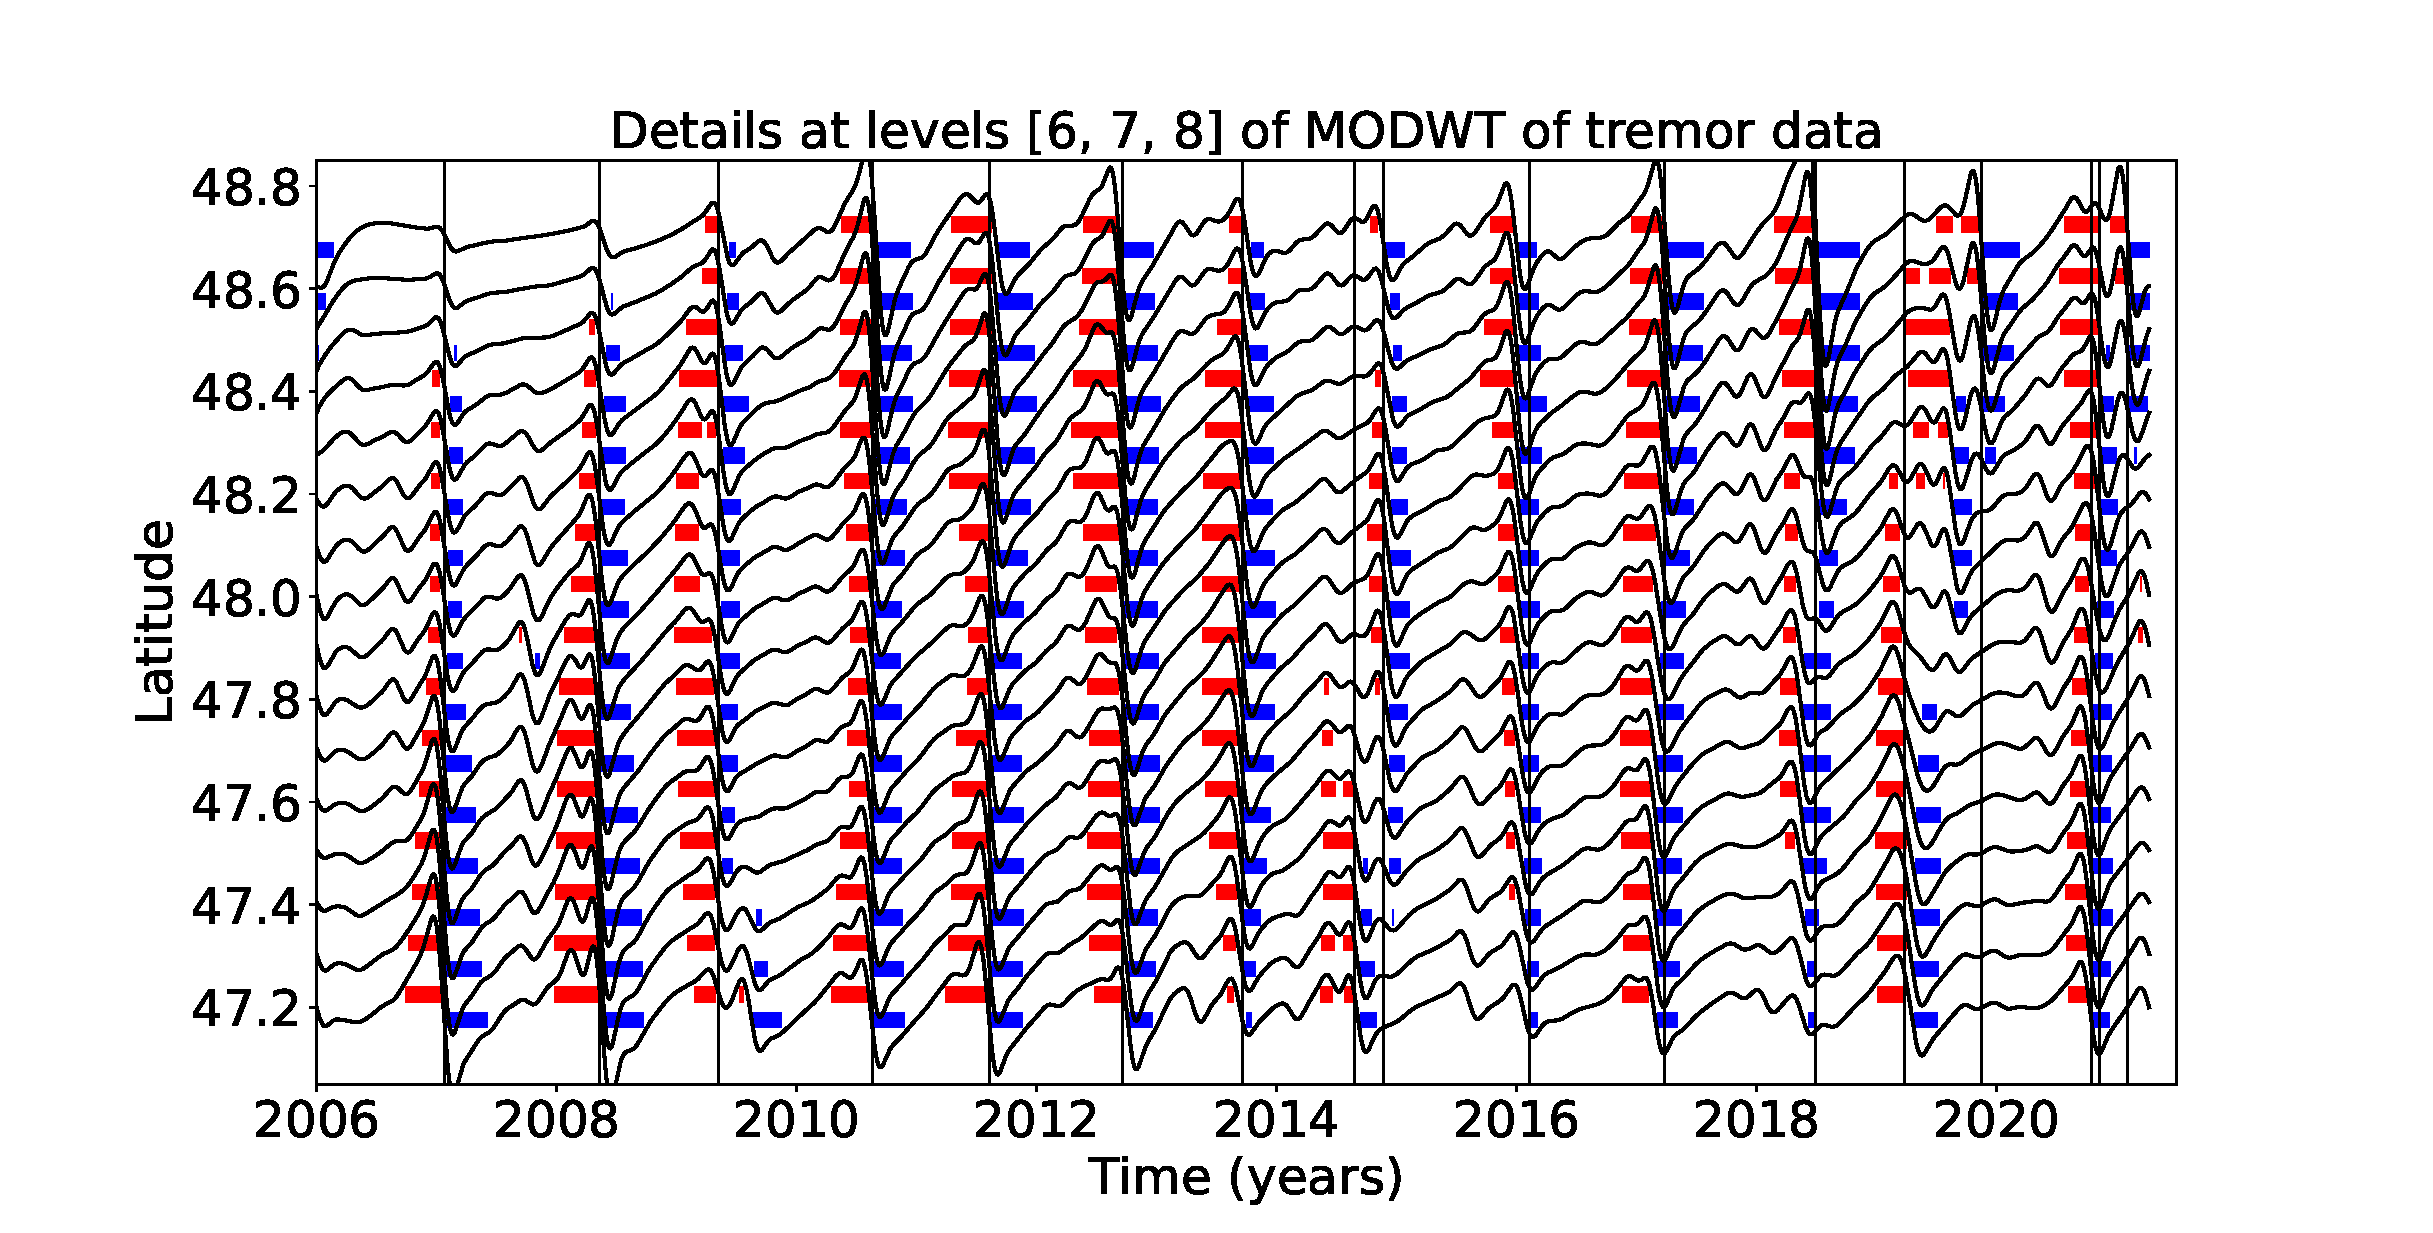
\includegraphics[width=\textwidth, trim={0cm 0cm 0cm 0cm},clip]{figures/tremor_longer_detail_6-7-8.eps}
\caption{Same as Figure 6 but for the sum of the 6th, 7th and 8th level details. The thresholds are 0.8 (for the GPS) and 0.01 (for the tremor).}
\label{pngfiguresample}
\end{figure}

\begin{figure}
\noindent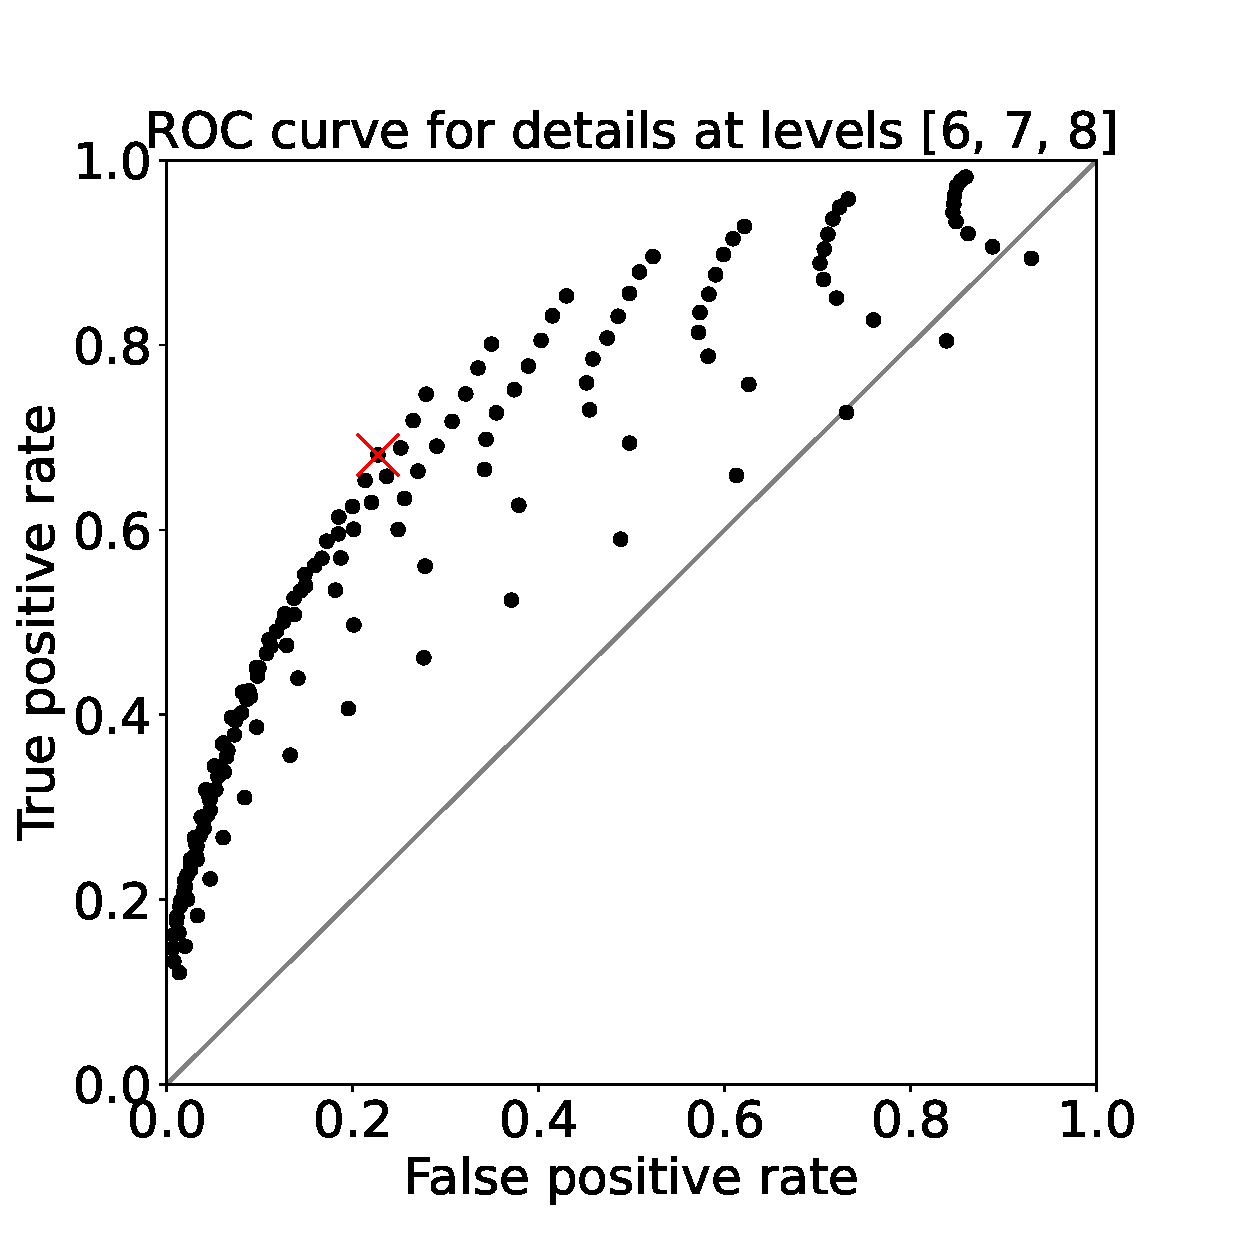
\includegraphics[width=\textwidth, trim={0cm 0cm 0cm 0cm},clip]{figures/ROC_6-7-8.eps}
\caption{ROC curve for the sum of the 6th, 7th, and 8th level details of the wavelet decomposition. Each black dot represents the true positive rate of event detections and the false positive rate of event detections for a given pair of thresholds (for the GPS and for the tremor). The red cross marks the true positive rate and the false positive rate obtained with the thresholds used to make Figure 9.}
\label{pngfiguresample}
\end{figure}

\begin{figure}
\noindent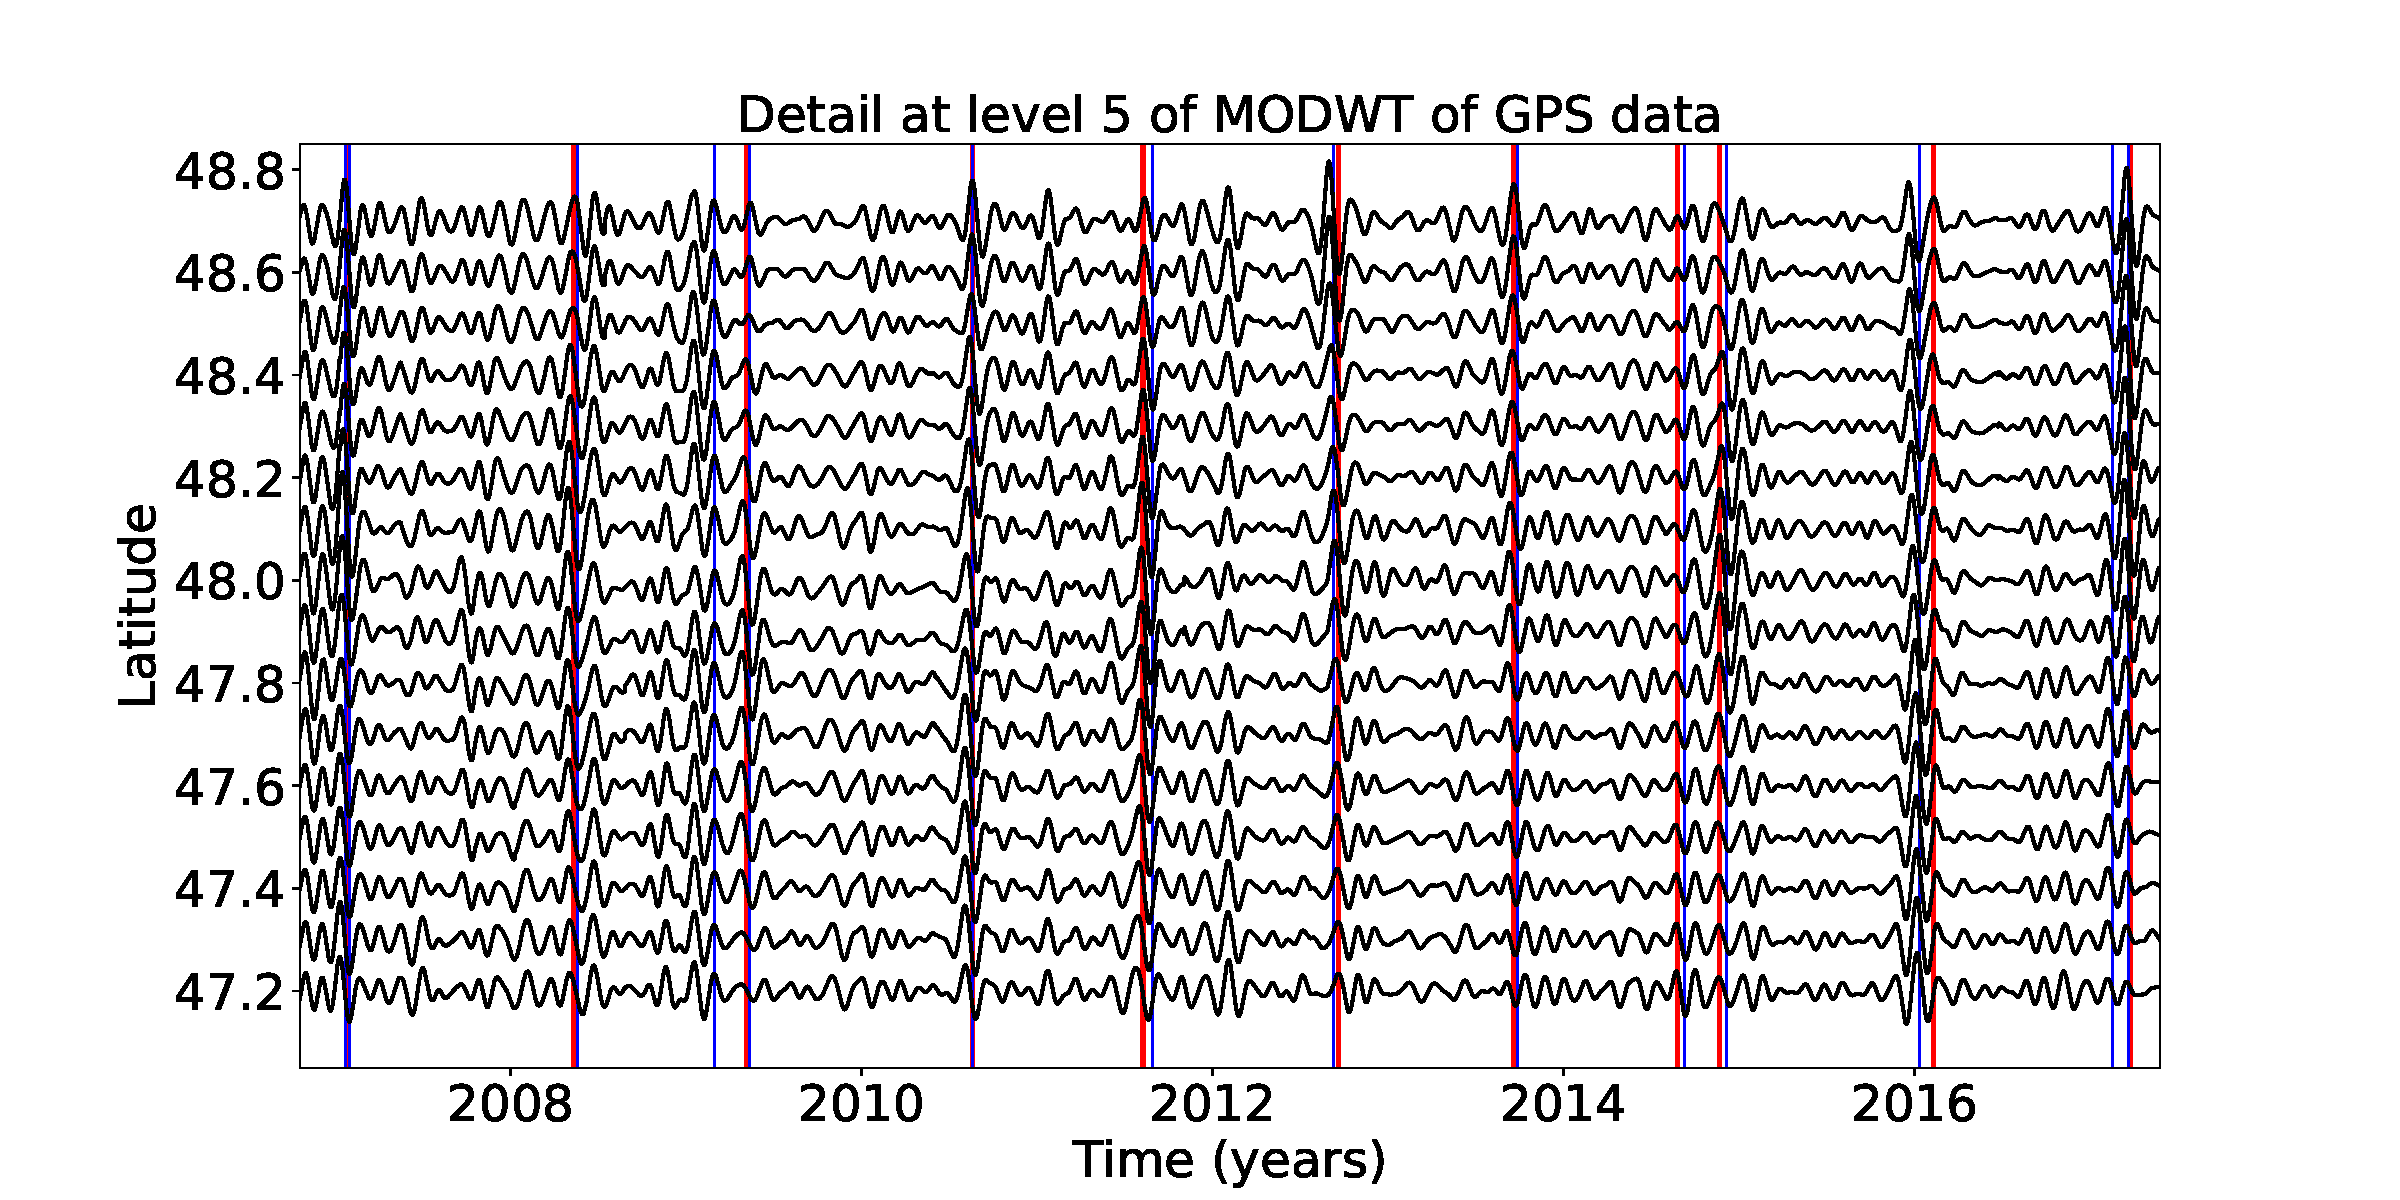
\includegraphics[width=\textwidth, trim={0cm 0cm 0cm 0cm},clip]{figures/GPS_michel_detail_5.pdf}
\caption{Top: Stacked 5th level details of the wavelet decomposition of the displacement over all the GPS stations located in a 50 km radius of a given point, for the 16 red triangles indicated in Figure 3. The red lines represent the timings of the ETS events from Table 1. The blue lines represent the timings of the magnitude 5 events from the catalog of ~\citet{MIC_2019}.}
\label{pngfiguresample}
\end{figure}

\end{document}
